\documentclass[
  oneside,
  11pt, a4paper,
  footinclude=true,
  headinclude=true,
  cleardoublepage=empty,
  bibliography=totocnumbered
]{scrbook}

\usepackage{dissertation}
\usepackage[utf8]{inputenc}
\usepackage[T1]{fontenc}
\usepackage{float}
\usepackage{indentfirst}
\usepackage{url}
\usepackage[toc]{appendix}
\usepackage{pgfplots, pgfplotstable}
\usepackage{fancyvrb}
\usepackage{makecell}
\usepackage{array}
\usepackage{subfig}
\usepackage[none,htt]{hyphenat}
\usepackage{listings}
\usepackage[cache=false]{minted}
\usepackage{amsmath}
\usepackage{caption}
\usepackage{array,tabularx}
\usepackage{cases}
\usepackage[ruled,vlined,linesnumbered]{algorithm2e}
\usepackage{vector}
\usepackage{mathtools}

\DeclarePairedDelimiter\ceil{\lceil}{\rceil}
\DeclarePairedDelimiter\floor{\lfloor}{\rfloor}

\SetKwInOut{Input}{input}
\SetKwInOut{Output}{output}

\newcommand{\var}{\texttt}
\newcommand\mycommfont[1]{\footnotesize\ttfamily\textcolor{blue}{#1}}

\SetCommentSty{mycommfont}

% ACRONYMS -----------------------------------------------------

%import the necessary package with some options
\usepackage[acronym,nonumberlist,nomain]{glossaries}

%enable the following to avoid links from the acronym usage to the list
\glsdisablehyper

%displays the first use of an acronym in italic
\defglsdisplayfirst[\acronymtype]{\emph{#1#4}}

%the style of the Glossary
\glossarystyle{listgroup}

% set the name for the acronym entries page
\renewcommand{\glossaryname}{Glossary}

%this shall be the last thing in the acronym configuration!!
\makeglossaries

%\loadglsentries[\acronymtype]{acronyms}

\newenvironment{conditions*}
{\par\vspace{\abovedisplayskip}\noindent
	\tabularx{\columnwidth}{>{$}l<{$} @{\ : } >{\raggedright\arraybackslash}X}}
{\endtabularx\par\vspace{\belowdisplayskip}}

\DeclareCaptionType{MyEquation}[][List of equations]
\captionsetup[MyEquation]{labelformat=empty}

\lstset{
	float=H,
	breaklines=true,
	breakatwhitespace=false,
	keepspaces=true,
	keywordstyle=\color{blue},
	numbers=left,
	showlines=true,
	stepnumber=1,
	stringstyle=\color{red},
	tabsize=2,
	frame=single,
	columns=fullflexible,
	language=C++,
	basicstyle=\small,
	keywordstyle=\color{blue}\ttfamily,
	stringstyle=\color{red}\ttfamily,
	commentstyle=\color{magenta}\ttfamily,
}

\sloppy

\AtBeginEnvironment{minted}{\dontdofcolorbox}
\def\dontdofcolorbox{\renewcommand\fcolorbox[4][]{##4}}

\newenvironment{conditions}
{\par\vspace{\abovedisplayskip}\noindent\begin{tabular}{>{$}l<{$} @{${}={}$} l}}
	{\end{tabular}\par\vspace{\belowdisplayskip}}

\graphicspath{ {Images/} }

% ----------------------------------------------------------------

% Title
\titleA{Mobile Ray Tracing}

% Author
\author{Tiago Manuel da Silva Santos}

% Supervisor(s)
\supervisor{Professor Doutor Luís Paulo Peixoto dos Santos}

% Date
\date{\myear} % change to text if date is not today

% Keywords
%\keywords{master thesis}

% Glossaries & Acronyms
\makeglossaries  %  either use this ...
%\makeindex	   % ... or this

% Define Acronyms
\newacronym{mei}{MEI}{Mestrado em Engenharia Informática}
\newacronym{di}{DI}{Departamento de Informática}
\newacronym{um}{UM}{Universidade do Minho}
\newacronym{qos}{QoS}{Quality of Service}
\newacronym{soa}{SOA}{Service Oriented Architecture}
\newacronym{api}{API}{Application Programming Interface}
\glsaddall[types={\acronymtype}]

\ummetadata % add metadata to the document (author, publisher, ...)

\begin{document}
% Cover page ---------------------------------------
\umfrontcover
\umtitlepage
	
% Add acknowledgements ----------------------------
\chapter*{Acknowledgements}

\par
Agradeço a todos que me apoiaram, direta ou indiretamente, neste longo percurso académico.
Em especial, ao meu orientador, professor Doutor Luís Paulo Peixoto dos Santos que propôs
este tema, deu-me sempre boas ideias e por todo o seu apoio.
Também, ao professores dos perfis de Computação Gráfica e de Computação Paralela e Distribuída pela excelente formação que deram.

\par
A todos os meus amigos que sempre me apoiaram neste longo percurso.
Em especial, destaco cinco amigos: João Costa, André Pereira, Miguel Esteves, Eduardo Mendes e Miguel Rego que desde que os conheci me ajudaram muito a ultrapassar diversos obstáculos tanto a nível pessoal como na minha formação académica.

\par
Ao grupo Embedded Systems Research Group (ESRG) por me terem acolhido durante uma bolsa de investigação, me tratarem como parte dessa grande família e pelo apoio que sempre me deram.

\par
E por último mas não menos importante, à minha família, em especial aos meus irmãos Pedro Santos e Paulo Santos pelos muitos sacrifícios que fizeram para me apoiar e permitir chegar onde cheguei.

% Add abstracts (en,pt) ---------------------------
\chapter*{Abstract}

\par
The technological advances and the massification of information technologies have allowed a huge and positive proliferation of the number of libraries and APIs.
This large offer has made life easier for programmers in general, because they easily find a library, free or commercial, that helps them solve the daily challenges they have at hand.

\par
One area of information technology where libraries are critical is in Computer Graphics, due to the wide range of rendering techniques it offers.
One of these techniques is ray tracing.
Ray tracing allows to simulate natural electromagnetic phenomena such as the path of light and mechanical phenomena such as the propagation of sound.
Similarly, it also allows to simulate technologies developed by men, like Wi-Fi networks.
These simulations can have a spectacular realism and accuracy, at the expense of a very high computational cost.

\par
The constant evolution of technology allowed to leverage and massify new areas, such as mobile devices.
Devices today are increasingly faster and replace and / or complement tasks that were previously performed only on computers or on dedicated hardware.
However, the number of image rendering libraries available for mobile devices is still very scarce, and no ray tracing based image rendering library has been able to assert itself on these devices.
This dissertation aims to explore the possibilities and limitations of using mobile devices to execute rendering algorithms that use ray tracing, such as progressive path tracing.
Its main goal is to provide a rendering library for mobile devices based on ray tracing.

\chapter*{Resumo}

\par
Os avanços tecnológicos e a massificação das tecnologias de informação permitiu uma enorme e positiva proliferação do número de bibliotecas e APIs.
Esta maior oferta permitiu facilitar a vida dos programadores em geral, porque facilmente encontram uma biblioteca, gratuita ou comercial, que os ajudam a resolver os desafios diários que têm em mãos.

\par
Uma área das tecnologias de informação onde as bibliotecas são fundamentais é na Computação Gráfica, devido à panóplia de métodos de renderização que oferece.
Um destes métodos é o ray tracing.
O ray tracing permite simular fenómenos eletromagnéticos naturais como os percursos da luz e fenómenos mecânicos como a propagação do som.
Da mesma forma também permite simular tecnologias desenvolvidas pelo homem, como por exemplo redes Wi-Fi.
Estas simulações podem ter um realismo e precisão impressionantes, porém têm um custo computacional muito elevado.

\par
A constante evolução da tecnologia permitiu alavancar e massificar novas áreas, como os dispositivos móveis.
Os dispositivos são hoje cada vez mais rápidos e cada vez mais substituem e/ou complementam tarefas que anteriormente eram apenas realizadas em computadores ou em hardware dedicado.
Porém, o número de bibliotecas para renderização de imagens disponíveis para dispositivos móveis é ainda muito reduzido e nenhuma biblioteca de renderização de imagens baseada em ray tracing conseguiu afirmar-se nestes dispositivos.
Esta dissertação tem como objetivo explorar possibilidades e limitações da utilização de dispositivos móveis para a execução de algoritmos de renderização que utilizem ray tracing, como por exemplo, o path tracing progressivo.
O objetivo principal é disponibilizar uma biblioteca de renderização para dispositivos móveis baseada em ray tracing.
	
% Summary Lists ------------------------------------
\tableofcontents
\listoffigures
\listoftables
\listofalgorithms
\printglossary[type=\acronymtype, style=long]
\clearpage
\thispagestyle{empty}

\pagenumbering{arabic}

% Chapter - Introduction -------------------------
% CHAPTER - falar do aumento do numero e da capacidade dos dispositivos moveis
% CHAPTER - falar da oportunidade de poder avaliar algoritmos de ray tracing nos dispositivos moveis
\chapter{Introduction}

\section{Context}

\par
%Identify the problem
Programming is like building something with primitive blocks and it can be a very difficult task if we have to program every aspect of the application without some “blocks” already built for us to use.
That’s why in the programming world there is a whole panoply of free and commercial libraries with APIs that provide a huge quantity of functions for the programmer to use.

\par
In computer graphics, there are many 3D graphics libraries that provide functionalities to render images based in different techniques.
Two of the most used render techniques are rasterization and ray tracing.
Ray tracing can be used to calculate and simulate the path of particles and waves.
It can simulate the propagation of sound, the path of light and even allows to simulate technologies developed by men like the Wi-fi networks.
It can render an image by tracing the path of light through pixels in an image plane and simulating the effects of its interactions with virtual objects.
It can render much more realistic shadows, reflections and refractions and in an easier way than rasterization.
This technique is capable of producing a very high degree of visual realism but at a great computational cost.

\par
Since nowadays we have more and more mobile systems whose computational power increases every year, the need for more libraries to help the programmers develop applications for these systems is increasing too.
However, there are not many options to choose from for developing a renderer based on ray tracing.
That’s why this dissertation focuses on assessing and providing a ray tracer library for mobile systems.

\par
%To delimit the problem
It is important to mention that this dissertation is not focused on rendering techniques other than ray tracing.
It is not focused in assess different integrators (numerical solutions to the rendering equation) and / or assess different approaches in ray tracing like Packet Traversal.
It is also not focused on assess different quasi random numbers generators neither assess the performance of different computer systems.

\par
These rendering algorithms based in ray tracing are very useful because they allow rendering photo-realistic images with a degree of realism much better than the graphics cards allow by default through rasterization.
As previously stated, the computing power in mobile devices processors has been increasing and this may allow a mobile device with a mid-range processor to run these algorithms in a useful time.

\begin{figure}[H]
\centering
\caption{Illustration of the most common mobile devices - tablet and smartphone (\cite{JournalDuNet}).}
\label{Illustration of the most common mobile devices - tablet and smartphone}
\includegraphics[width=10cm,height=10cm,keepaspectratio,scale=1.0]{Mobile_devices.jpg}
\end{figure}

\section{Motivation}

\par
Among other factors, the productivity of a programmer depends on what libraries he can have access to.
But, there are almost no rendering libraries based in ray tracing available today for mobile systems like Android, iOS, Windows 10 Mobile, BlackBerry 10, Tizen, Sailfish OS, Symbian and Ubuntu Touch.
And it is likely that these systems already have enough processing power to render images with fairly complex scenes in an acceptable time by using algorithms based in ray tracing.

\par
It is also important to note that there is not much documentation about the advantages and limitations of executing different rendering algorithms in these devices.

\par
Last but not least, it is important to mention that of all the operating systems available for mobile devices, the one chosen for this ray tracing library was Android.
Because nowadays it is the operating system with the most market share.
More than 85\% of the mobile devices use Android, and only 14\% of these devices use iOS which is the second most used operating system in these devices.
And, besides that, it allows to be executed on a variety of different devices: smart phones, tablet computers, smart TVs, smart watches and even laptop / desktop computers.

\begin{figure}[H]
	\centering
	\caption{Illustration of a variety of mobile devices compatible with Android (\cite{AndroidDevices}).}
	\label{Illustration of a variety of mobile devices compatible with Android}
	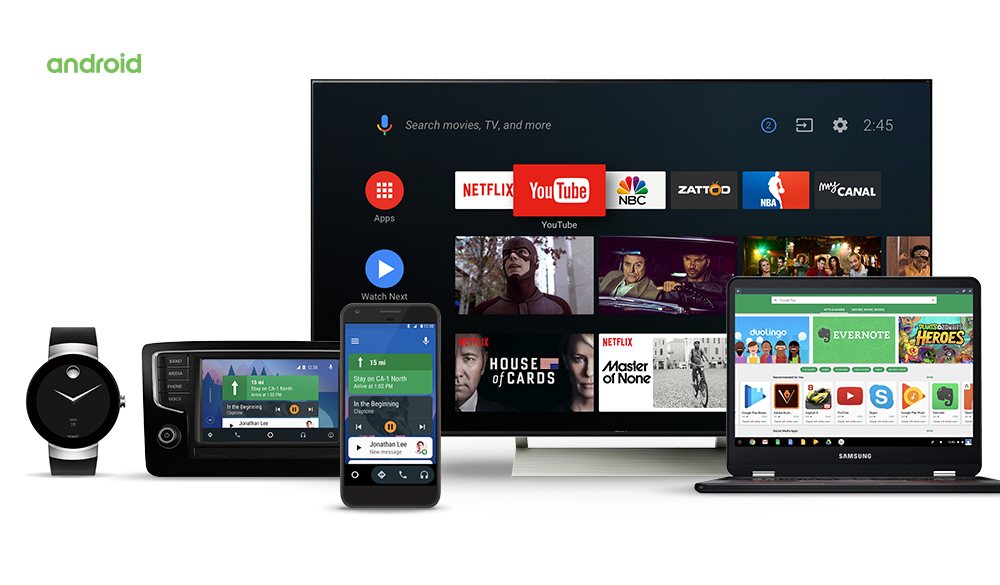
\includegraphics[width=10cm,height=10cm,keepaspectratio,scale=1.0]{Android_devices.png}
\end{figure}


\section{Goals}

\par
The main goal of this dissertation is to assess and demonstrate the advantages of running rendering algorithms in mobile devices.

\par
It is also intended to promote and facilitate the development of applications for mobile systems that use ray tracing techniques, with special emphasis on rendering applications.
To do this, it will be developed a library that supports the fundamental operations of a ray tracing engine.
This library will allow the agile development of diverse applications, by using components that invoke the functionality of the library itself.

\par
Additionally, it is intended to supply rendering components at a higher abstraction level, like the camera, scene and the integrator that facilitates further the development of applications.

\par
Finally, it is important to do a demonstration of the rendering application with some interface layer to let the user assess the performance of several functionalities provided by the library.

\section{Applications of Ray Tracing}

\par
The subject of this dissertation is about ray tracing because it is a technology widely used in several areas of Computer Graphics.

\par
Ray tracing is a rendering technique that is widely used in the areas of theater and television lighting.
It allows set and lighting designers, actors, and directors to develop and visualize complex lighting setups months before a production ever opens.

\par
Ray tracing is capable of considering all of the light in a given environment which is called Global Illumination.
Global illumination is a physically correct model, which accurately simulates light's behavior in a real physical environment.
Global illumination is a valuable engineering tool in that it allows us to quantitatively analyze the distribution and directionality of light and research radiant heat transfer.

\par
Finally, ray tracing can also be used in the Animation market.
It can be used to add "fancy" effects such as reflection and shadowing that are often difficult and time consuming for traditional artists to produce.
Graphical technology is also capable of rendering photo-realistic images that would be nearly impossible to produce without computerized ray tracing.


\section{Document Structure}

\par
This dissertation is organized in six chapters: Introduction, State of the Art, Software Architecture, Android challenges, Demonstration: Global Illumination and Conclusion \& Future work.

\par
The first chapter describes the context and motivation behind this work, as well as its goals.
Its main purpose is to identify the problem at hand and set up goals that should be accomplished.

\par
The second chapter introduces the main concepts of ray tracing and compares different implementations of ray tracers already available in the world wide web.
The reason behind this comparison is to show how many ray tracers are already available to mobile devices and highlight the differences between the features they provide.
It also provides some information about the processors of today that helps realize their ability to execute computationally demanding algorithms like ray tracing.

\par
The third chapter explains the proposed approach and explains each module developed in the library, as well as each of the rendering components.

\par
The fourth chapter starts with an explanation of some Android specifics, such as the user interface by characterizing its work flow and mentioning some of the benefits and challenges overcame during the development of the application.
It also describes some programming decisions made during the development of the ray tracing library.

\par
The fifth chapter summarizes the key results obtained by executing different algorithms with different number of threads and different acceleration structures.
And concludes with a small comparison of the features provided in this library and an Android ray tracing engine developed by third parties called Android CPU Raytracer (\cite{Android_CPU_Raytracer}).

\par
Finally, the last chapter ends this dissertation with the conclusions that can be withdrawn from this work and proposes some future work.

\par
Last but not least, the Appendix contains this library's API and an example code of how to load a scene from a wavefront obj file.

% Chapter - State of the Art ---------------------
% CHAPTER - falar de diferentes arquiteturas de ray tracing
% ou
% CHAPTER - falar de diferentes ports de apps para android
\chapter{State of the art}

\section{Ray Tracing}

\par
Ray tracing one frame can be, simultaneously, a computationally demanding task and an embarrassingly parallel task.
As tracing rays is a recursive process which aims to calculate the luminance of light of each individual pixel separately.
At least one ray is shot per pixel and in a naive approach each ray would be intersected with all the objects in the scene in order to determine which one is the closest primitive intersecting that given ray.
To evaluate the light intensity that an object scatters towards the eye, the intensity of the light reaching that object has to be evaluated as well.
Ray tracing achieves this by shooting additional secondary rays, because when a ray hits a reflecting or transparent surface, one or more secondary rays are cast from that point, simulating the reflection and refraction effects.

\begin{figure}[H]
	\centering
	\caption{Illustration of a typical ray tracer algorithm.}
	\label{Illustration of a typical ray tracer algorithm.}
	\includegraphics[keepaspectratio,scale=0.3]{Ray_Tracing.png}
\end{figure}

\par
A typical image of 1024 x 1024 pixels tends to cast at least a million primary rays and a multiple of that as shadow, reflection, refraction and secondary rays.
This is why ray tracing can't provide interactive frame rates with ease.

\section{Typical CPU features}

\par
Fortunately, the present state of available technology provides affordable machines with multiple CPU cores that can work in parallel and with great performance.
This is achieved thanks to features developed inside the processor like the cache, the multilevel pipeline, the hardware prefetching and SIMD instruction set already available in the current processors.

\par
The cache is a very small and fast multilevel memory inside the processor that temporarily stores the data read from the main memory.
This memory allows reading its content at a very low latency in the order of magnitude of around 1 nanosecond in the first level, 10 nanoseconds at second level and 50 nanoseconds at third level compared to the typical 100 nanoseconds of a DDR main memory.
The downside is that it is very small because its cost are much higher than a typical RAM memory.
Nowadays, the level 1 has 64kB, the level 2 has 256kB and the level 3 has 8 MB which is very little compared to the typical 16GB provided by the memory RAM.

\begin{figure}[H]
	\centering
	\caption{Illustration of a typical cache memory inside a microprocessor (\cite{CPU_Cache}).}
	\label{Cache.}
	\includegraphics[keepaspectratio,scale=0.3]{cache.png}
\end{figure}

\par
The multilevel pipeline is another feature inside a processor which allows to reduce the processor's own latency by allowing a form of parallelism called instruction-level parallelism within a single processor.
Basically, one instruction is divided in some stages and it allows the possibility to execute different stages of different instructions simultaneously.
In the early days, the Classic RISC pipeline were typically divided in five stages:
\begin{itemize}  
	\item Fetching the instruction
	\item Decoding the instruction
	\item Executing the instruction where the arguments can be fetched from registers (1 cycle latency) or from memory (2 cycle latency)
	\item Memory access where it ensured that writing in memory was always performed in the same stage and allowed to use that value in another instruction before it was written in memory
	\item Writing back the value in the register
\end{itemize}
Nowadays, the current microprocessors have a pipeline with 8-14 stages and can be more complex than the Classic RISC, but the operating principle is the same.
This allows faster CPU throughput, which means the number of instructions that can be executed in a unit of time is greater, than it would otherwise be possible at a given clock rate.

\begin{figure}[H]
	\centering
	\caption{Illustration of the Classic RISC multilevel CPU pipeline (\cite{CPU_Pipeline}).}
	\label{Pipeline.}
	\includegraphics[keepaspectratio,scale=0.5]{Pipeline.png}
\end{figure}

\par
The hardware prefetching is, as the name implies, a feature in the processor that makes the processor fetch the data and the instructions before it really needs to execute.
This allows to reduce the time that the processor waits for the data in the main memory.

\par
Finally, SIMD instruction set is a set of special instructions that allows the processor to read or write bigger sizes of data.
Typically, a 64 bit processor can only work with 64 bits of information at a time during the execution of an instruction.
This feature can allow to read or write up to 512 bits by using special registers and additional ALUs provided in the processor.

\begin{figure}[H]
	\centering
	\caption{Illustration of a typical execution of SIMD extension (\cite{CPU_SIMD}).}
	\label{SIMD.}
	\includegraphics[keepaspectratio,scale=0.5]{SIMD.png}
\end{figure}

\par
Nowadays, even mobile devices like smart phones and tablets have multiple CPU cores with features similar to those described above.
This opens the possibility to execute more computationally demanding algorithms, like ray tracing, in these devices.

\section{Key features of Ray Tracing for this work}

\par
Ray tracing is an algorithm that can have a panoply of features or optimizations in order to reduce the time required to trace all the rays and / or to show the results as fast as possible.
It also, like any application, can have different types of software licenses and be executed in different platforms.

\par
For this work, the most important features in a ray tracer are: the type of software license, the platform where can be executed, interactivity, progressive and the type of rendering components.

\subsection{Type of software license}

\par
A software application can have different type of software license, but in order to simplify this dissertation, the software license were grouped into three types: Free, Commercial and Open Source.
The license Free means that the user has the right to execute freely the application but cannot copy, modify or distribute the implemented code.
The license Commercial means that the user cannot even execute the application without buying it first and cannot copy, modify or distribute the implemented code.
The license Open Source means that the user has the right to execute freely the application and can even copy, modify and distribute the implemented code.
The software license is very important in this work because it lets the user know if he can develop something over the provided software or if he can just use the application.

\subsection{Platform}

\par
An application can only be executed in the platforms that the developers compiled the code for.
So, a ray tracer that can be executed in a desktop may also or may not be executed on another platform, like a mobile device.
This information is very important in this work because it inform us whether a ray tracer can be executed in a mobile device with the typical Operating System like Android, iOS or Windows 10 Mobile.

\subsection{Interactivity}

\par
In ray tracing, interactivity means rendering an image with a very low response time, like a few milliseconds per frame.
An interactive ray tracer can render a scene with multiple frames per second.

\subsection{Progressive}

\par
A typical ray tracer shows the rendered image only after the whole process is complete.
A progressive ray tracer is a ray tracer that updates the color of pixels in the screen as soon as the rays are traced, instead of waiting for the rendering process to complete.
This means that an image is rendered quickly with some aliasing or noise and it is progressively improved over time.

\subsection{Types of Rendering Components}

\par
A ray tracer can be developed with the different rendering components programmed separately.
Some examples of rendering components are: Integrators, Cameras, Scenes, Samplers, Shapes, Lights and Accelerator Structures.
In some ray tracers, these rendering components can even be programmable by the user.
This is very important because it allows the user to develop his own renderer based in ray tracing without having to develop every feature in the ray tracer.

\section{Related work}
\label{RelatedWork}

\par
The possibility of rendering an image with ray tracing was demonstrated in 1980 by Whitted (\cite {RT_classic}) and since then the number of libraries that provide basic ray tracing functionalities increased greatly.
There is a wide range of different ray tracers available today for the programmer to use, yet the majority can only be used with the traditional personal computer hardware (desktop or laptop).

\par
The table \ref{comparison state of the art} shows some applications or frameworks that use ray tracing available today and compares them according to their type of license, platform compatibility, interactivity, progressive and whether they allow development of your own rendering components like the integrator and sampler.
Note that some of these ray tracers provide only the engine with the basic ray tracing functions, such as creating rays and intersecting them with geometric primitives, so the rendering components are only programmable if the application that uses the engine supports it.
During the research of the available ray tracers, others than the ones presented in the table were found, but they were excluded because the documentation was very poor without explaining the basic functionalities provided or because there was no documentation at all.

\begin{table}[H]
\centering
\caption{Comparison of different applications/frameworks that use ray tracing.}
\label{comparison state of the art}
\hspace*{-2.0cm}
\scriptsize
\begin{tabular}{|c|c|c|c|c|c|c|c|}
\hline
\textbf{Product}											& \textbf{License}	& \textbf{Platform}	& \textbf{Mobile}		& \textbf{Interactivity}	& \textbf{Progressive}	& \makecell{\textbf{Programmable} \\ \textbf{Components}}\\ \hline
Optix (\cite{Optix})											& F                	& Nvidia GPU 			& N				& Y                  	& Y                 		& Y\\ \hline
Optix Prime (\cite{OptixPrime})								& F                	& CPU \& Nvidia GPU 	& N				& Y                  	& Y                 		& Y\\ \hline
RenderMan RIS (\cite{RIS})									& C       	& CPU 		             & N                  		& Y                 		& Y				& Y\\ \hline
OctaneRender (\cite{OctaneRender})							& C       	& GPU 		             & N                  		& Y                 		& Y				& N\\ \hline
Embree (\cite{Embree}										& O     	& Intel CPU			& N				& Y                  	& Y                      	& Y\\ \hline
Radeon Rays (\cite{RadeonRays})							& O	& CPU \& GPU		& N				& Y                    	& Y                     	& Y\\ \hline
PBRT (\cite{PBRT})	 									& O	& CPU				& N                 		& N                 		& N				& N\\ \hline
Visionaray (\cite{Visionaray})									& O     	& CPU \& Nvidia GPU	& N                  		& Y				& Y                  	& N\\ \hline
YafaRay	(\cite{YafaRay})									& O     	& CPU 				& N                  		& N				& N                  		& N\\ \hline
tray\_rust (\cite{trayrust})									& O    	& CPU                  	& N                   	& N                  		& N                 		& N\\ \hline
micro-packet (\cite{micro-packet})							& O     	& Intel CPU 			& N                  		& N                  		& N 				& N\\ \hline
tray (\cite{tray})											& O     	& CPU 				& N				& N                     	& N                  		& N\\ \hline
The G3D Innovation Engine (\cite{G3D17})						& O	& CPU 				& N				& N                 		& N                 		& N\\ \hline
HRay (\cite{HRay})										& O     	& CPU                		& N                  		& N                      	& N				& N\\ \hline
Mitsuba (\cite{Mitsuba})										& O 	& CPU 				& N				& N                 		& N				& N\\ \hline
Indigo RT (\cite{IndigoRT})									& O 	& CPU \& GPU		& N				& Y                 		& N				& N\\ \hline
jsRayTracer (\cite{jsRayTracer})								& O 	& CPU 				& N				& Y                 		& Y				& N\\ \hline
Android CPU Raytracer (\cite{Android_CPU_Raytracer})			& O 	& CPU 				& Y (Android)		& Y                 		& N				& N\\ \hline
\end{tabular}
\normalsize
\end{table}

\subsection{Conclusions}

%Em que é que o que eu proponho é diferente das anteriores.

\par
As the table \ref{comparison state of the art} shows, there is a lack of generic ray tracing libraries for the mobile devices.
Although there are some closed-source ray tracing demo applications, only one ray tracer already available has some sort of documentation and is compatible with mobile devices, in this case with Android.
This ray tracer is open source, uses only the CPU of the device and has a good performance.
It even allows interactions with the objects during the render process.
But, it doesn’t support progressive rendering and also does not allow the programmers to use their own rendering components.

\par
This dissertation aims to fix this lack of libraries, by providing one that contains ray tracing basic functionalities and the ability to let the programmer be able to develop their own rendering components like the sampler, integrator, camera and shapes of virtual objects.
It also studies the drawbacks that these mobile devices may have comparing with the average multi-core personal computer hardware.
And finally, a small comparison was made with the Android CPU Raytracer (\cite{Android_CPU_Raytracer}) in order to illustrate the advantages and disadvantages of both.
This comparison is important because it enriches all the work done, as it demonstrates if the performance of the provided features are relatively efficient.

% Chapter - Ray Tracing -------------------------
% CHAPTER - desenhar diagrama de classes
% CHAPTER - explicar a implementaçao da lib
% CHAPTER - explicar a implementaçao dos componentes
% CHAPTER - falar da dependencia stdlib do C++
\chapter{Software architecture}

\section{Approach}

\par
The development of this demonstration application involves the distinction of three layers of abstraction: user interface, rendering components and the library itself.

\par
The top layer is the User Interface which is obviously application, and eventually device, dependent.
The user interface of this dissertation's demo application is very simple and just allows the user to see the rendered image and choose some rendering components to use, like the integrator, the sampler, the number of threads and samples and choose the scene to render.
Although this layer is useful, this dissertation focuses only on the middle and bottom layers.

\begin{figure}[H]
	\centering
	\caption{Illustration of the developed User Interface.}
	\label{UI.}
	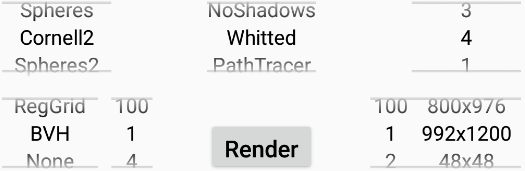
\includegraphics[width=10cm,height=10cm,keepaspectratio,scale=1.0]{UI.png}
\end{figure}

\par
The middle layer provides the rendering components, which are abstract concepts about rendering, that use functionalities that the library itself offers to the programmers.
Some of these rendering components are the camera, the light, the sampler, the integrator and the object loader.
These rendering components are useful for the programmer since it allows them to use features without having the need to know how these were developed.
And, of course, this facilitates and accelerates the development of new rendering applications for the programmers.

\par
Lastly, the bottom layer is the library itself, which contains the business logic of basic features in a renderer, that the rendering components use.
These features are the basic functionalities of a ray tracing engine.
Those functionalities can be: create vectors and points; create different shapes like triangles, spheres and planes; create different primitives with different materials and with different shapes; cast rays; and even intersect rays with the primitives.

\par
It is also important to mention that the demo application was built in order to show the developed features, the performance achieved in the mobile devices and also to help promote the library.
This demo application is a good way to test it in several Android devices, like: a smart phone, a tablet computer, a smart TV, or even a smart watch.

\begin{figure}[H]
	\centering
	\caption{Illustration of the three layers in the application.}
	\label{Illustration of the three layers in the application.}
	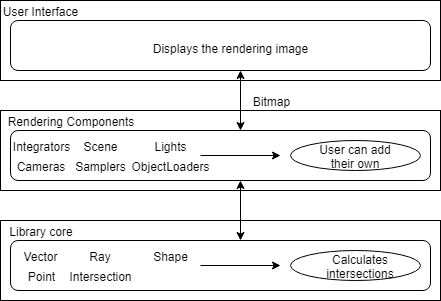
\includegraphics[width=10cm,height=10cm,keepaspectratio,scale=1.0]{Layers.png}
\end{figure}

\par
Besides the abstraction layers, there are some important strategic decisions made in order to guide the progress of the development of this library.

\par
The first decision was: the primary rays always have origin in the camera.
This decision was made in order to not mix the code of the integrator with the ray tracer renderer engine.

\par
Other decision made was to make the rendering process progressive, which means that the rendered image is incrementally refined with more and more traced rays.
As the integrator will be converging to better values.
This is important in order to give the user a fast rendered image, with some noise or aliasing, and converge it progressively to a better solution with higher details and practically without any visual noise or aliasing.

\par
Last, but not least, is that the code was developed in a modular way, in this case was programmed in an object oriented manner.
This allows the programmers to code their own rendering components, like the integrator, camera, sampler and light, without having to develop the basic features in the renderer engine.

\section{Methodology}

\par
In order to take advantage of most of the mobile CPU resources and give a good performance for the applications, the library and the rendering components were developed using the native programming language C++.
This was achieved by using the Native Development Kit (NDK) provided by the Integrated Development Environment (IDE) Android Studio.
This way, the mobile device can provide better performance in computationally intensive applications because it doesn't need the Java garbage collector.
And it facilitates the porting of existing C/C++ code to Android and promotes developing multi-platforms applications.
But, it won't ensure device portability despite processor architecture and the number of libraries compatible with the NDK is very scarce.
It is also important to mention that the User Interface was developed in Java using the traditional Software Development Kit (SDK) provided by the Android Studio because there is no framework in the NDK that helps the programmer design his own User Interface.
Despite that, its performance is not very important because it doesn't interfere significantly with the others layers of the application.



\iffalse

\section{Work plan}

\par
The development of this dissertation will be done in six stages.

\par
The first stage involves the survey of state of the art about ray tracers built for mobile systems, in order to understand the capacities and limitations of these devices when running rendering algorithms.

\par
The second stage is to make the requirements specification in order to:

\begin{itemize}
\item Describe the functionalities of the library.
\item Explain how the user interact with the external interfaces.
\item Demonstrate the design constraints imposed on an implementation of a custom rendering component.
\end{itemize}

\par
The third stage will address the development of the architecture of the entire system.
The study performed in the previous stages will serve as the basis for this development, where this architecture should be able to address all the possible problems that might arise in the development process.

\par
The fourth stage will be the development and test of the software, where it should be relatively quick if the previous stage was done properly.

\par
Next it will be made a demo application in order to illustrate the possibilities and limitations of this rendering process in the mobile devices.

\par
Finally, the writing of this dissertation will be done throughout the entire project, but there will be a reinforced effort at the end along with the writing of an article.

\par
In short, the work plan of this dissertation should be as follows:

\begin{enumerate}

\item Survey of the State of the Art (2 weeks)
\item Requirements specification (2 weeks)
\item Development of Software Architecture (3 months)
\item Development and test of the library (2 weeks)
\item Development of a demonstration (2 weeks)
\item Writing the dissertation and an article (1 month)

\end{enumerate}

\begin{table}[H]
\centering
\caption{Scheduling for this dissertation}
\label{Scheduling for this dissertation}
\begin{tabular}{|c|c|c|c|c|c|c|}[H]
\hline
\textbf{}                               & \multicolumn{6}{c|}{\textbf{2017}} \\ \hline
                                        & Jan  & Feb & Mar & Apr & May & Jun \\ \hline
Survey of the State of the Art          & X    &     &     &     &     &     \\ \hline
Requirements specification              & X    &     &     &     &     &     \\ \hline
Development of Software Architecture    &      & X   & X   & X   &     &     \\ \hline
Development and test of the library     &      &     &     &     & X   &     \\ \hline
Development of a demonstration          &      &     &     &     & X   &     \\ \hline
Writing the dissertation and an article &      &     &     &     &     & X   \\ \hline
\end{tabular}
\end{table}

\fi



\section{Library}

\par
As stated above, this library was implemented in an object-oriented fashion.
The most important classes that provide functionalities already developed for the user to use are:

\begin{itemize}
\item Renderer: class that starts the rendering process and stores the calculated pixels colors in a C style array.
\item Scene: class that stores the geometry information in vectors and provides methods to trace rays in the scene without any acceleration structures.
\item Shapes: set of classes that allows to create triangles, spheres and planes.
\item Material: class that stores all four types of material color:
\begin{itemize}
	\item Emission light color
	\item Diffuse reflection color
	\item Specular reflection color
	\item Specular refraction color
\end{itemize}
\item Primitive: class that stores the shape and material of each primitive in the scene.
\item Ray: class that represents a ray casted into the scene.
\end{itemize}

\subsection{Third parties dependencies}

\par
Before describing each functionality provided in each class developed, it is important to mention that this library uses four other libraries developed in C++ by third parties.
Those libraries are:

\begin{itemize}
	\item OpenGL Mathematics (\cite{GLM}): used to create 3d points and vectors, perform geometry calculations and store pixels and primitives' colors.
	Before using this library, it was implemented our own mathematics library and its performance was very bad compared with this library.
	\item tinyobjloader (\cite{tinyobjloader}): used to load scenes from wavefront obj files into the main memory.
	\item Google Test (\cite{GoogleTest}): used to create some unit tests and to mock some classes.
	This is important in order to have a safe and maintainable code.
	\item C++ Standard Library (\cite{C++_stdlib}): used in order to save the data in popular containers like the array and the vector.
	It also provides some useful utilities like the unique pointers in the Dynamic memory management utilities, the String and the Atomic operations used in the Samplers.
\end{itemize}

\par
All these libraries are Android compatible and are reliable in terms of performance and maintenance.
Besides being dependent on these four libraries, this library also depends on OpenGL ES 2.0 (\cite{OpenGL_ES_2}) from Android SDK and depends on CMake (\cite{CMake}) in order to compile the application.

\par
The OpenGL ES 2.0 is necessary in order to let the application rasterize one frame of the scene so the user can view it without having to wait a long time to render it with the ray tracer.
For example, in the Conference scene, the OpenGL in the Samsung Galaxy Fresh Duos can rasterize one frame in less than 17ms compared with 500ms that the NoShadows shader takes.
This is done by copying the scene data from native code to the OpenGL of JVM with the help of JNI.

\begin{figure}[H]
	\centering
	\caption{The Conference scene rendered with OpenGL ES 2.0 before ray tracing the scene.}
	\label{The Conference scene rendered with OpenGL ES 2.0 before ray tracing the scene.}
	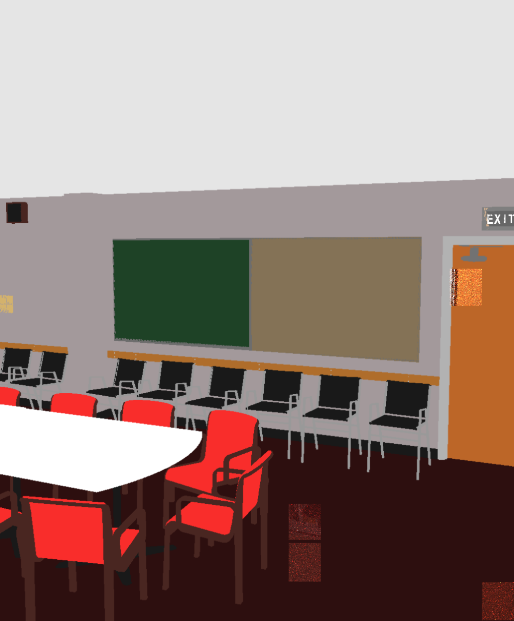
\includegraphics[width=10cm,height=10cm,keepaspectratio,scale=1.0]{OpenGL_Conference.png}
\end{figure}

\par
The CMake was used so that the application code could be compiled on any operating system.
As it is a cross-platform family of tools designed to build, test and package software developed for a variety of operating systems like Windows, Linux, Mac OS X, and even FreeBSD.
The main goal of CMake is to control the software compilation process using simple platform and compiler independent configuration files, and generate native makefiles and workspaces that can be used in the compiler environment of the programmer's choice.
This facilitates the integration of third party libraries that use CMake to compile into our own project.
But, unfortunately the NDK only provides CMake up to the version 3.6.0, so projects that use latter versions of CMake will not work.

\par
The CMake generate makefiles that call the available C++ compilers in the Android Environment.
The NDK in Android Studio uses, by default, the LLVM Project, which is a collection of modular and reusable compiler and toolchain technologies.
This toolchain provides Clang, which is C/C++/Objective-C compiler that aims to deliver amazingly fast compiles and extremely useful error and warning messages for the programmers.
Unfortunately, this compiler only provides features up to C++ 17, so developers can't use the most recent features of C++ 20.

\par
Last, but not least, it is important to mention that all the code of this application, including the ray tracer library, the rendering components and the Graphical User Interface are available in the github, which is a web-based hosting service for version control using Git.
It is 100\% open source and it is accessed in the web page:
\url{https://github.com/PTPuscas/MobileRayTracer}.

\subsection{Renderer}

\par
The Renderer is the closest class to the application that starts the rendering process.
This class provides two main methods:

\begin{lstlisting}[caption={Main methods in Renderer}, captionpos=b, label=Renderer]
void renderFrame(std::uint32_t *bitmap, std::int32_t numThreads, std::uint32_t stride) noexcept;
void stopRender() noexcept;
\end{lstlisting}

\par
The \textit{renderFrame} method starts the rendering process and writes the calculated light luminance of each pixel in the array parameter \textit{bitmap}.
This method also allows to choose the number of threads that will render the image into the bitmap, and needs the \textit{stride} of that bitmap array.
Besides rendering the scene in a progressive way, the image plane is divided into 256 tiles of pixels and it is traced one primary ray per pixel in each tile.
This allows the user to wait less time in order to view the scene being rendering.

\begin{figure}[H]
	\centering
	\caption{Illustration of tiling the image plane.}
	\label{Illustration of tiling the image plane.}
	\includegraphics[width=10cm,height=10cm,keepaspectratio,scale=1.0]{tiling.png}
\end{figure}

\par
The \textit{stopRender} method only serves to stop the rendering process without resetting the pixels' colors already calculated.

\subsection{Scene}

\par
The Scene is the class that handles the process of intersecting a ray with the primitives and source lights in the scene.
Besides providing a vector to add the light sources and a vector to add primitives to the scene, it also provides two main methods:

\begin{lstlisting}[caption={Main methods in Scene}, captionpos=b, label=Scene]
Intersection trace(Intersection intersection, const Ray &ray) noexcept;
Intersection shadowTrace(Intersection intersection, const Ray &ray) noexcept;
\end{lstlisting}

\par
The \textit{trace}, as the name implies, is a method that tries to intersect a ray with all the primitives and light sources in the scene.
And it returns the closest intersection to the origin of that ray.
This method is used to determine the intersection of the casted ray with the primitives in the scene.

\par
The \textit{shadowTrace}, is similar to the \textit{trace} method but with the difference that returns the first intersection found.
The purpose of this method is to simulate the shadows in the scene, like it is illustrated in figure \ref{Illustration of shadow rays casting.}.
The shadow ray is represented by the yellow line pointed to the light source.

\begin{figure}[H]
	\centering
	\caption{Illustration of shadow rays casting (\cite{ShadowRays}).}
	\label{Illustration of shadow rays casting.}
	\includegraphics[width=10cm,height=10cm,keepaspectratio,scale=1.0]{Shadow_Ray.jpg}
\end{figure}


\subsection{Shapes}

\par
In order to make possible to generate scenes with all kind of objects, it was developed three types of shapes: plane, sphere and triangle.

\par
One way to allow this would be to use the process of inheritance available in C++.
Which means, for example, create a class called Shape and create sub classes like Triangle, Plane or Sphere that are derived from that class.
And each of those classes would implement different intersect methods.
In this way, it would be possible for the programmer to develop his own custom shapes as new Rendering Components.
But of course, the benefit of this flexibility also brings the downside of performance loss as the application will have at runtime to figure out which of the derived classes is required to call.
Because, calling a virtual function requires a v-table lookup, and can make it 2-3 times slower than a normal function.

\par
The other way to do it is by developing each shape class without inheritance and being each class independent of each other.
This can have greater performance but the downside is that the programmer cannot add new shapes to the library.
This ray tracer was implemented this way because it is not important to let the user add his own custom shapes as rendering components.
Because with only the triangles it is possible to render many types of custom shapes.
Also, the performance is critical in the intersect method of the shapes because it is a method that can be called millions of times while rendering a scene.

So, all shapes provide three important methods:

\begin{lstlisting}[caption={Main methods in Shape}, captionpos=b, label=Shape]
Intersection intersect(const Intersection &intersection, const Ray &ray) const noexcept;
bool intersect(const AABB &box) const noexcept;
AABB getAABB() const noexcept;
\end{lstlisting}

The first
$intersect$
method determines if a ray intersects the shape and returns the corresponding intersection.
It is important to mention that, obviously, each shape was developed with different algorithms.

The second
$intersect$
method checks if an AABB contains the shape, and only returns true or false.
This is useful to determine in which AABB the shape belongs to in the regular grid accelerator.

Finally, the
$getAABB$
method, as the name implies returns the smallest AABB that surrounds the shape.
This is used in the building of the acceleration structures because it allows to check if a ray intersects multiple shapes inside an AABB.
And it is simpler to intersect an AABB than a shape.

\subsubsection{Plane}

\par
The plane is an essential primitive shape because it allows the user to build indoor scenes.

\par
The construction of a plane requires just an arbitrary point in the plane and the normal of the plane.
So, the intersect method implemented has the following algorithm taken from \cite{RayPlane}:

Let
\begin{equation}
\label{intersectionPlane}
\begin{aligned}
intersectionPoint = rayOrg + rayDir * dist \\
n \cdot (q - x) = 0 \\
n \cdot (q - intersectionPoint) = 0 \\
n \cdot (q - rayOrg - rayDir * dist) = 0 \\
n \cdot (q - rayOrg) = (n \cdot rayDir) * dist \\
dist = [ n \cdot (q - rayOrg) ] / (n \cdot rayDir) \\
\end{aligned}
\end{equation}

where
\begin{conditions*}
	n  &  normal of the plane \\
	q  &  known point on the plane \\
	x  &  any point on the plane \\
	rayOrg & origin of the ray \\
	rayDir & direction of the ray \\
	dist & distance of the ray \\
	intersectionPoint  &  intersection point of the ray in the plane \\
\end{conditions*}


\begin{figure}[H]
	\centering
	\caption{Illustration of a ray intersecting a plane (\cite{PlaneRayIntersection}).}
	\label{Plane.}
	\includegraphics[keepaspectratio,scale=0.4]{RayToPlane.png}
\end{figure}

\par


\subsubsection{Sphere}

\par
The sphere is also an important primitive shape because it allows the user to build some common objects with a shape of a ball.

\par
The construction of a sphere requires just the point in the center and the radius of the sphere.
It also should be noted that a ray can intersect a sphere at two points and therefore it is necessary to determine the closest intersection point to the origin of the ray.
The algorithm used in this library was the algebraic version.
So, the intersect method implemented has the following algorithm taken from \cite{RaySphere}:

Let
\begin{equation}
\label{intersectionSphere}
\begin{aligned}
intersectionPoint = rayOrg + rayDir * dist \\
dist=\frac{-b\pm\sqrt{b^2-4ac}}{2a} \\
\end{aligned}
\end{equation}
where
\begin{conditions*}
	a  &  $\|rayDir\| ^ 2$ \\
	b  &  $2 * rayOrgToCenter \cdot rayDir$ \\
	c  &  $\|rayOrgToCenter\| ^ 2 - sphereRadius ^ 2$ \\
	rayOrgToCenter & vector from the origin point of the ray to the center of the sphere \\
	sphereRadius & radius of the sphere \\
	sphereCenter & center point of the sphere \\
	rayOrg & origin point of the ray \\
	rayDir & direction of the ray \\
	dist & distance of the ray \\
	intersectionPoint  &  intersection point of the ray in the sphere \\
\end{conditions*}

\begin{figure}[H]
	\centering
	\caption{Illustration of a ray intersecting a sphere in two points (\cite{SphereRayIntersection}).}
	\label{Sphere.}
	\includegraphics[keepaspectratio,scale=0.4]{Ray_Sphere_Intersection.png}
\end{figure}

\subsubsection{Triangle}

\par
And finally, obviously the triangle has also been implemented because, as it is the simplest primitive with an area, it allows to build many different object shapes.
The implemented Ray-Triangle Intersection algorithm was the Möller-Trumbore (\cite{RayTriangleIntersection}) algorithm, which was named after its inventors Tomas Möller and Ben Trumbore.

\par
The construction of a triangle requires three points
$[A, B, C]$
, two vectors
$[AB, AC]$
and the normal of the triangle.
This is needed in order to execute the Möller-Trumbore algorithm  for the intersection of a ray with a triangle.
The Möller–Trumbore ray-triangle intersection algorithm is a fast method for calculating the intersection of a ray and a triangle in three dimensions without the needing to precompute the plane equation containing the triangle.
It only needs to store 1 triangle vertex and 2 triangle vectors, which means that each triangle needs only to store 9 floating point values, or 36 bytes.
So, the intersect method implemented has the following algorithm:

Let
\begin{equation}
\begin{aligned}
\label{intersectionTriangle}
intersectionPoint = rayOrg + rayDir * dist \\
dist = (AC \cdot ((rayOrg - A) * AB)) / (AB \cdot (rayDir * AC)) \\
\end{aligned}
\end{equation}

where
\begin{conditions*}
	A & point A of the triangle \\
	AB & vector of the triangle from point A to B \\
	AC & vector of the triangle from point A to C \\
	rayOrg & origin point of the ray \\
	rayDir & direction of the ray \\
	dist & distance of the ray \\
	intersectionPoint  &  intersection point of the ray in the triangle \\
\end{conditions*}

\begin{figure}[H]
	\centering
	\caption{Illustration of a ray intersecting a triangle (\cite{TriangleRayIntersection}).}
	\label{Sphere.}
	\includegraphics[keepaspectratio,scale=1.0]{triangle.png}
\end{figure}

\subsection{Acceleration Structures}

\par
As previously stated, the rendering algorithms based on ray tracing can be very computationally demanding, like Path Tracing and Bidirectional Path Tracing.
These algorithms are very computationally demanding because if the scene is very complex, made with millions of primitives, it is necessary to try to intersect every ray casted into the scene with those millions of primitives.
This task is, obviously, very time consuming and can waste a lot of battery power on the mobile device.
Luckily, there are already known techniques, called acceleration structures, that helps to accelerate this process by reducing the number of intersections.

\par
There are two types of approaches that acceleration structures can have:

\begin{itemize}
	\item Subdivision of Space: the 3D space of the scene is divided into smaller portions of space which each volume element can be uniform or irregular:
	\begin{itemize}
		\item Regular Grids
		\item Octrees
		\item Kd-trees
	\end{itemize}
	\item Subdivision of Objects: the 3D space of the scene is divided by aggregating the 3D primitives in groups which are next to each others:
	\begin{itemize}
		\item Bounding Volume Hierarchy (BVH)
	\end{itemize}
\end{itemize}

\par
The idea in Subdivision of Space is allowing the intersections to start with the nearest primitives of the ray and is only intersected with the further ones, if the closest ones are not in the same direction of the ray.
These structures also allow the rapid and simultaneous rejection of groups of primitives.

\par
In contrast, structures based on Subdivision of objects only allow the rapid and simultaneous rejection of groups of primitives.

\par
The developed library provides only two types of structures, one of each approach: the regular grid and the bounding volume hierarchy.
Both structures are built with Axis Aligned Bounding Volumes (AABB), which are volume elements (voxels) that can cover, one or more primitives from the 3D scene.
An AABB is a voxel, like the name implies, that is aligned to the axis of the scene.
This type of voxels are great to use in acceleration structures because it is very fast to test whether or not a ray intersects that voxel and it only needs to store, in memory, two points of that box.
Besides AABB, it is possible to build the structures with other types of voxels, like:

\begin{itemize}
	\item Sphere: intersection with a sphere is simpler than AABB but covers more 3D space than the scene primitive needs.
	\item Oriented Bounding Volume: its like an AABB but rotated according to the orientation of the primitive.
	\item k-Discrete Oriented Prototype (k-DOP): a generalization of AABBs defined by k hyperplanes with normals in discrete directions.
	\item Convex Hull: is the smallest and more complex convex volume containing the object.
\end{itemize}

\subsubsection{Regular Grid}

\par
A regular grid is an acceleration structure where the scene space is subdivided into equal voxels.
Each voxel is a volume element where it could have inside one or more primitives of the scene, if a ray intersects that voxel, then it tries to intersect the primitives inside it.
The order of testing each voxel is from the nearest of the ray into the furthest in the direction of that ray.
This type of structure is very fast to build but its traversal is poorly efficient due to poor distribution of primitives by voxels.
The figure \ref{RegularGrid.} shows the process of intersecting a ray with the primitives in a scene.

\begin{figure}[H]
	\centering
	\caption{Illustration of traversing a regular grid acceleration structure (\cite{RegularGrid}).}
	\label{RegularGrid.}
	\includegraphics[keepaspectratio,scale=1.0]{Regular_Grid.jpg}
\end{figure}

\par
The developed ray tracer library provides a regular grid as an acceleration structure and its trace operation is as shown in the figure \ref{RegularGrid.}.

\subsubsection{Bounding Volume Hierarchy}

\par
Bounding Volume Hierarchy is another acceleration structure provided in the developed library.
This structure is different from the regular grid because the space is not divided into voxels of the same size.
The space is divided in a way where the primitives of the scene are grouped according to the nearest primitives of each.
This allows to build a structure of voxels where each voxel has, for sure, one or more primitives inside.

\par
The figure \ref{BVH.} shows an example of a BVH structure of a scene.
As it can be seen, each primitive is covered by an AABB, and then two or more AABBs are covered by one larger AABB.
In this library, this is built in a top down manner, where the scene is divided by a fake plane that divides the scene into two AABBs.
The calculation of those planes is performed with the Surface Area Heuristic (SAH) algorithm which is a very popular heuristic commonly used in ray tracers.

\begin{figure}[H]
	\centering
	\caption{Illustration of traversing a Bounding Volume Hierarchy acceleration structure (\cite{BVH}).}
	\label{BVH.}
	\includegraphics[keepaspectratio,scale=1.0]{BVH.jpg}
\end{figure}

\par
In this library, the BVH class is a template, because this way, it is possible to create multiple BVH classes where each one store a vector of primitives with different shapes.

\subsubsection{Surface Area Heuristic}

\par
As it was said above, the library uses the Surface Area Heuristic in order to split the scene.
The algorithm used in the library is very simple, it just needs to calculate the minimum area surface of the sum of left and right sub-trees, as following:

\begin{equation}
SAH_{optimal} = min(S_L * N_L + S_R * N_R)
\end{equation}

\begin{conditions}
	N_L & number of polygons in left subtree \\
	N_R & number of polygons in right subtree \\
	S_L & surface area of left subtree \\
	S_R & surface area of right subtree \\
\end{conditions}

\par
The figure \ref{SAH.} shows a very simple example of how the SAH algorithm works.

\begin{figure}[H]
	\centering
	\caption{Illustration of how Surface Area Heuristic works in Bounding Volume Hierarchy acceleration structure (\cite{SAH}).}
	\label{SAH.}
	\includegraphics[keepaspectratio,scale=1.0]{SAH_example.png}
\end{figure}

\subsection{Primitive}

\par
The Primitive is a template class that needs a Shape and wraps it with the Material together.
It is useful to be a template class because this way it allows to different shapes have different types of material.

\begin{lstlisting}[caption={Main methods in Primitive}, captionpos=b, label=Primitive]
Intersection intersect(Intersection intersection, const Ray &ray) noexcept;
AABB getAABB() const noexcept;
\end{lstlisting}

\par
The \textit{intersect}, as the name implies, is a method that tries to intersect a ray with the primitive.
This method calls the \textit{intersect} of the Shape and it returns the closest intersection to the origin of that ray.
It is used to determine the intersection of the casted ray with the primitives in the scene.

\par
The \textit{getAABB} is the method that returns the AABB voxel that surrounds the primitive as it just returns the call of \textit{getAABB} from the Shape.
It is used to construct the Acceleration Structures.


\section{Rendering Components}

\par
In order to show the functionalities provided by the library, it was developed a few Rendering Components.
It is provided the perspective and orthographic cameras, the area and point lights, six Samplers, five Shaders and one Object loader.

\subsection{Shaders}

\par
The implemented ray tracer was programmed in an objected oriented fashion, so each Rendering Component was developed separately, in a different class.
This allows the user to develop his own Rendering Components without having to develop the ray tracer engine.

\par
A shader is the most important Rendering Component because it is the Rendering Component that describes how the Rendering Equation is approximated.
The Rendering Equation describes how the total radiance reflected by any point
$p$
of a surface in a direction
$\omega$$r$
is calculated.
The Bidirectional Reflectance Distribution Function (BRDF) is a function that tries to approximate the Rendering Equation.
In summary, a shader, in this context, is the algorithm of a BRDF.

\begin{figure}[H]
	\centering
	\caption{Illustration of the rendering equation describing the total amount of light emitted from a point
	$x$
	along a particular viewing direction and given a function for incoming light and a BRDF (\cite{RenderingEquation}).}
	\label{Rendering_Equation.}
	\includegraphics[width=10cm,height=10cm,keepaspectratio,scale=1.0]{Rendering_eq.png}
\end{figure}

\par
There were developed five shaders: NoShadows, Whitted, PathTracer, DepthMap and DiffuseMaterial.
All shaders provide only one main method that allows the user to calculate the RGB color of a pixel with the information of a ray casted into the scene and its nearest calculated intersection.
This method was implemented differently in each shader.
Besides that method, the class Shader provides three other important methods that all shaders have access to:

\begin{lstlisting}[caption={Main methods of Shader}, captionpos=b, label=Shader]
virtual bool shade(glm::vec3 *rgb, const Intersection &intersection, const Ray &ray) noexcept = 0;
glm::vec3 getCosineSampleHemisphere(const glm::vec3 &normal) const noexcept;
bool rayTrace(glm::vec3 *rgb, const Ray &ray) noexcept;
bool shadowTrace(Intersection intersection, const Ray &ray) noexcept;
\end{lstlisting}

\par
The method
$shade$
calculates the color of the pixel that will be stored in the parameter
$rgb$
and the
$intersection$
contains the calculated information about the intersection of a ray with the nearest primitive of the scene like the intersection point, its normal and the material of the intersected material.
Finally the parameter
$ray$
is where the information about the ray like its origin and its direction is accessed.

\par
The method
$getCosineSampleHemisphere$
calculates a random direction in World coordinates around an hemisphere with a given
$normal$.
This method is used to cast new secondary rays in the scene in order to simulate the indirect light.
This is typically used in Path Tracers.

\subsubsection{DepthMap}

\par
DepthMap is a very simple shader that calculates an image or image channel that contains information relating to the distance of the surfaces of scene objects from a viewpoint (\cite{DepthMap}).
It is useful to various things like simulating the effect of uniformly dense semi-transparent media within a scene, such as fog, smoke or large volumes of water; or even to create Shadow Maps.

The algorithm is as much as simple as:

\begin{algorithm}
	\small
	\label{DepthMap}
	\caption{Algorithm of DepthMap Shader}
	\Input{\var{maxPoint}, \var{rayOrigin},\var{intersectionLength}}
	\Output{\var{outputRGB}}
	
	$\var{maxDist} \gets ||\var{maxPoint} - \var{rayOrigin}||$ \\
	$\var{depth} \gets (\var{maxDist} - \var{intersectionLength}) / \var{maxDist}$ \\
	$\var{outputRGB} \gets [\var{depth}, \var{depth}, \var{depth}]$ \\
\end{algorithm}

%where
%\begin{conditions*}
%	maxPoint & is the furthest 3D point that the user send as parameter in the DepthMap constructor \\
%	rayOrigin & origin point of the ray \\
%	intersectionLength & the distance from the origin of the ray to the intersection point  \\
%	outputRGB & the output parameter to write the pixel's RGB color \\
%\end{conditions*}

%Where the
%$maxPoint$
%is the furthest 3D point that the user send as parameter in the DepthMap constructor.

\begin{figure}[H]
	\centering
	\caption{DepthMap shader.}
	\label{DepthMap shader.}
	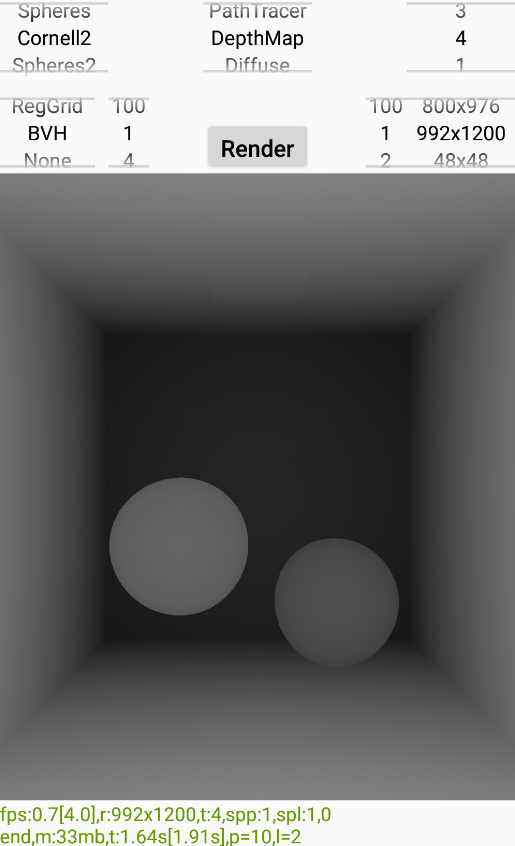
\includegraphics[keepaspectratio,scale=0.3]{DepthMap.png}
\end{figure}


\subsubsection{DiffuseMaterial}

\par
The DiffuseMaterial is another very simple shader that only computes directly the diffuse material color of the intersected primitive.
But, in case the primitive material does not have diffuse color, the specular color is computed or the transmission color or even the light emission.
This is can be useful to debug the application because it renders the scene, including all types of materials, very fast.
And the algorithm is very simple as illustrated below:

\begin{algorithm}
	\small
	\label{DiffuseMaterial}
	\caption{Algorithm of DiffuseMaterial Shader}
	\Input{\var{kD}, \var{kS}, \var{kT}, \var{Le}}
	\Output{\var{outputRGB}}
	
	\eIf{\var{kD} > $0$}{
		$\var{outputRGB} \gets \var{kD}$ \\
	}{\eIf{\var{kS} > $0$}{
			$\var{outputRGB} \gets \var{kS}$ \\
		}{\eIf{\var{kS} > $0$}{
				$\var{outputRGB} \gets \var{kT}$ \\
			}{\uIf{\var{Le} > $0$}{
					$\var{outputRGB} \gets \var{Le}$ \\
				}
			}
		}
	}
\end{algorithm}

\begin{figure}[H]
	\centering
	\caption{DiffuseMaterial shader.}
	\label{DiffuseMaterial shader.}
	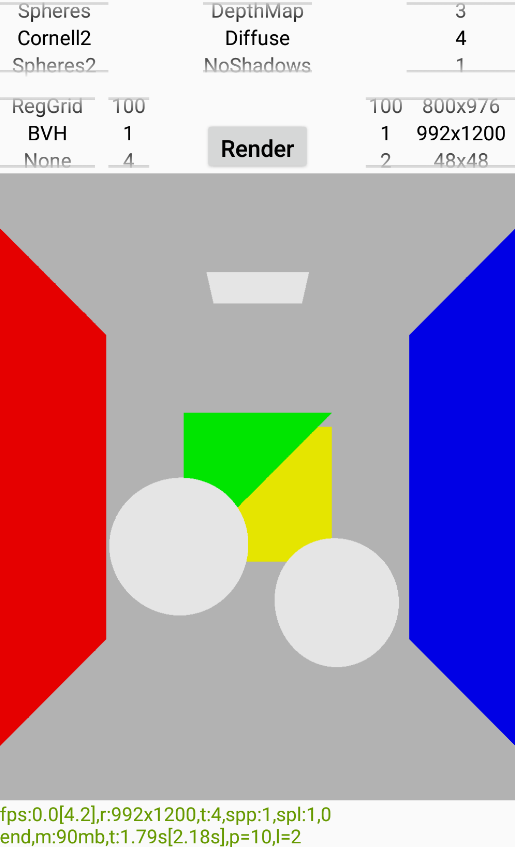
\includegraphics[keepaspectratio,scale=0.3]{DiffuseMaterial.png}
\end{figure}


\subsubsection{NoShadows}

\par
NoShadows is a simple shader because, as the name implies, it does not synthesize the shadows and it only simulates the direct lighting.
This BRDF only simulates direct lighting in primitives with diffuse surfaces and it does not take into account the light coming from other points.
As already said, the indirect lighting is not fully simulated but rather approximated with a fixed ambient light of about 10\% of the diffuse color of the objects.
This can be useful in order to let the user render a scene with good details and without having to wait as long as the Whitted algorithm.

\par
The algorithm developed is as following:

\begin{algorithm}
	\small
	\label{NoShadows}
	\caption{Algorithm of NoShadows Shader}
	\Input{\var{intersectionPoint}, \var{intersectionNormal}}
	\Output{\var{outputRGB}}
	
	\uIf{intersected material is diffuse}{
		\ForEach{light}{
			\ForEach{sample}{
				$\vec{vectorToLight} \gets \var{lightPos} - \var{intersectionPoint}$ \\
				$\var{cosNL} \gets \vec{vectorToLight} \cdot \vec{intersectionNormal}$ \\
				\uIf{\var{cosNL} > $0$}{
					$\var{outputRGB} \gets \var{outputRGB} + (\var{kD} * \var{radLight} * \var{cosNL})$ \\
				}
			}
		}
		$\var{outputRGB} \gets \var{outputRGB} / \var{\#samples}$ \\
		$\var{outputRGB} \gets \var{outputRGB} / \var{\#lights}$ \\
		$\var{outputRGB} \gets \var{outputRGB} + \var{kD} * 0.1$ \\
	}
\end{algorithm}

\begin{figure}[H]
	\centering
	\caption{NoShadows shader.}
	\label{NoShadows shader.}
	\includegraphics[keepaspectratio,scale=0.3]{NoShadows.png}
\end{figure}

\subsubsection{Whitted}

\par
As the name of this shader implies, Whitted is the algorithm presented by John Turner Whitted in the 1980s.
Like the previous shader, it doesn't simulate indirect lighting.
This BRDF recursively perform the ray casting to simulate refraction and reflection on diffuse and specular surfaces.
In order to simulate a reflective and refractive surfaces, the algorithm was divided into each case.
This makes it possible to simulate refractive surfaces, reflective surfaces and even refractive and reflective surfaces.

\par
The reflected light in a diffuse surface is calculated by adding the casting rays in direction to the lights.
These rays are called shadow rays and their radiance are multiplied by the dot product between vector to the light and the shading normal.
At the end, the summation is multiplied by the diffuse color of the intersected primitive and divided by the number of samples taken.

\par
The reflected light in a specular surface is calculated in a different way.
The specular ray is casted and ray traced, then the obtained radiance is multiplied by the specular color of the intersected primitive.
The reflection direction is the subtraction between the double of dot product between the inverse of the ray direction and the shading normal multiplying by the shading normal, and the inverse of the ray direction.

\begin{figure}[H]
	\centering
	\caption{Reflections projected on the floor and on the spheres (\cite{RTReflections}).}
	\label{Reflection.}
	\includegraphics[keepaspectratio,scale=0.3]{Reflection.png}
\end{figure}

\par
Finally, the refracted light in a transmission surface is calculated by using the refractive index of the intersected primitive and the ray direction and shading normal.

The specular refraction is calculated as follows:

\begin{algorithm}
	\small
	\label{Transmission}
	\caption{Algorithm of Specular Transmission}
	\Input{\var{rayDir}, \var{intersectionNormal}, \var{refractiveIndice}, \var{rayDepth}, \var{intersectionPoint}, \var{intersectionPrimitive},  \var{kT}}
	\Output{\var{specularTransmissionColor}}
	
	$\vec{refractDir} \gets glm::refract(\vec{rayDir}, \vec{intersectionNormal}, 1 / \var{refractiveIndice})$ \\
	$\var{transmissionRay} \gets Ray (\vec{refractDir}, \var{intersectionPoint}, \var{rayDepth} + 1, \var{intersectionPrimitive})$ \\
	$\var{LiT\_RGB} \gets rayTrace (\var{transmissionRay})$ \\
	$\var{specularTransmissionColor} \gets \var{kT} * \var{LiT\_RGB}$ \\
\end{algorithm}

\iffalse
First, the shading normal is inverted if the origin of the ray was inside a primitive, like a sphere, and if it was not then the refractive index is inverted.
Then, it is calculated two auxiliary scalar projections:
$cosTheta1$
and
$cosTheta2$
.
$cosTheta1$
is the dot product of the inverse of the shading normal and the ray direction, and
$cosTheta2$
is the difference of one and refractive index squared multiplied by one minus
$cosTheta1$
squared.
Then, if
$cosTheta2$
is greater than zero, then the direction of the transmission ray is ray direction multiplied with refractive index plus shading normal multiplied by refractive index multiplied $cosTheta1$
minus square root of 
$cosTheta2$
.
Else, the direction of the transmission ray is just ray direction plus shading normal multiplied by the double of
$cosTheta1$
.
\fi

And, as usual, the transmission ray is traced and its radiance is multiplied by the transmission component of the intersected primitive.

\begin{figure}[H]
	\centering
	\caption{Refraction of light at the interface of two media of different refractive indices (\cite{RTRefractions}).}
	\label{Refraction.}
	\includegraphics[keepaspectratio,scale=0.3]{Refraction.png}
\end{figure}

\par
The algorithm developed is as following:

\begin{algorithm}
	\small
	\label{Whitted}
	\caption{Algorithm of Whitted Shader}
	\Input{\var{rayDirection}, \var{intersectionNormal}, \var{refractiveIndice}, \var{rayDepth}, \var{intersectionPoint}, \var{intersectionPrimitive},  \var{kT}, \var{kS}}
	\Output{\var{outputRGB}}
	
	\uIf{intersected material is diffuse} {
		\ForEach{light}{
			\ForEach{sample}{
				$\vec{vectorToLight} \gets \var{lightPos} - \var{intersectionPoint}$ \\
				$\var{cosNL} \gets \vec{vectorToLight} \cdot \vec{intersectionNormal}$ \\
				\uIf{\var{cosNL} > $0$}{
					$\var{shadowRay} \gets Ray(\var{intersectionPoint}, \vec{vectorToLight}, \var{distanceToLight}, \var{rayDepth} + 1)$ \\
					\uIf{!shadowTrace (\var{shadowRay})}{
						$\var{outputRGB} \gets \var{outputRGB} + \var{radLight} * \var{cosNL}$ \\
					}
				}
			}
		}
		$\var{outputRGB} \gets \var{outputRGB} * \var{kD}$ \\
		$\var{outputRGB} \gets \var{outputRGB} / \var{\#samples}$ \\
	}

	\uIf{intersected material is specular reflective} {
		$\vec{reflectionDir} \gets glm::reflect(\vec{rayDir}, \vec{intersectionNormal})$ \\
		$\var{specularRay} \gets Ray(\vec{reflectionDir}, \var{intersectionPoint}, \var{rayDepth} + 1, \var{intersectionPrimitive})$ \\
		$\var{LiS\_RGB} \gets rayTrace(\var{specularRay})$ \\
		$\var{outputRGB} \gets \var{outputRGB} + \var{kS} * \var{LiS\_RGB})$ \\
	}
	
	\uIf{intersected material is specular refractive} {
		$\vec{refractDir} \gets glm::refract(\vec{rayDir}, \vec{intersectionNormal}, 1 / \var{refractiveIndice})$ \\
		$\var{transmissionRay} \gets Ray (\vec{refractDir}, \var{intersectionPoint}, \var{rayDepth} + 1, \var{intersectionPrimitive})$ \\
		$\var{LiT\_RGB} \gets rayTrace (\var{transmissionRay})$ \\
		$\var{outputRGB} \gets \var{outputRGB} + \var{kT} * \var{LiT\_RGB}$ \\
	}
\end{algorithm}

\begin{figure}[H]
	\centering
	\caption{Whitted shader.}
	\label{Whitted shader.}
	\includegraphics[keepaspectratio,scale=0.3]{Whitted.png}
\end{figure}


\subsubsection{PathTracer}

\par
Finally, the last developed shader is the canonical Path Tracer which is a Monte Carlo method of rendering images of three-dimensional scenes such that the global illumination is faithful to reality.
This renderer algorithm can synthesize very realistic scenes.
Unlike the previous shaders, this one fully simulates both direct and indirect lighting.
But, like the previous shader, this algorithm simulates the light reflected on diffuse and specular surfaces, as well as the light refracted on transparent primitives.

\par
The light reflected on diffuse surfaces is divided in two parts: direct lighting and indirect lighting.
The direct lighting is calculated in a similar way to the Whitted shader but with the difference that the samples are not taken from all sources of light but rather only one.
The light source in each sample is chosen randomly.
Then the obtained light radiance is multiplied by the Probability Density Function (PDF) in order to approximate the expected value.
In this case the PDF is as simple as
$1 / \#lights$.

\par
Finally, the indirect lighting reflected in diffuse surfaces is calculated in a much more complex way.
First it is generated, from the intersected point, a random direction on an unit hemisphere with a PDF proportional to cosine-weighted solid angle\\
($PDF: p(\Theta) = cos\theta / \pi$,
$x = cos(2\pi r1)\sqrt{1-r2}$,
$y = sin(2\pi r1)\sqrt{1-r2}$,
$z = \sqrt{r2}$)
.
This kind of PDF is one of the best ways to render images with path tracing that the rendering equation converges to the expected value as fast as possible.

Then to generate a new ray direction in a world coordinates from a hemisphere it is needed to distinguish the six different possible materials:

\begin{itemize}
	\item Diffuse reflection
	\item Glossy reflection
	\item Specular reflection
	\item Diffuse transmission
	\item Glossy transmission
	\item Specular transmission
\end{itemize}

\par
The figure \ref{Secondary_Rays.} illustrates those six possible scenarios.

To calculate the secondary ray direction in a diffuse reflective material, it was implemented a generator of random directions on unit hemisphere proportional to cosine-weighted solid angle around the normal of that hemisphere.
Sampling in a cosine weighted hemisphere is better than uniform sampling over the hemisphere about the normal because the rays casted at the bottom of the hemisphere will not contribute as much as the other directions because of the multiplication by the cosine of theta.

\par
To do this, it was implemented a method called \textit{getCosineSampleHemisphere}, which generates a random direction around an hemisphere oriented by an arbitrary normal.

\begin{lstlisting}[caption={Method in Shader which generates a random direction in an hemisphere.}, captionpos=b, label=Shader]
glm::vec3 getCosineSampleHemisphere(glm::vec3 normal);
\end{lstlisting}

\par
The algorithm to generate a random direction in an hemisphere was taken from  \cite{CosineSampleHemisphere}, which is as follows:

\begin{algorithm}
	\small
	\label{Shader}
	\caption{Method in Shader which generates a random direction in an hemisphere.}
	\Input{$\vec{normal}$}
	\Output{$\vec{newDir}$}
	
	$\var{phi} \gets 2 * \pi * \var{uniformRandom1}$ \\
	$\var{r2} \gets \var{uniformRandom2}$ \\
	$\var{cosTheta} \gets \sqrt{\var{r2}}$ \\
	$\vec{u} \gets \left| \var{normal.x} \right| > 0.1? [0,1,0] : [1,0,0]$ \\
	$\vec{u} \gets normalize(\vec{u} \times \vec{normal})$ \\
	$\vec{v} \gets \vec{normal} \times \vec{u}$ \\
	$\vec{newDir} \gets normalize(\vec{u} * (\cos(\var{phi}) * \var{cosTheta}) + \vec{v} * (\sin(\var{phi}) * \var{cosTheta}) + \vec{normal} * \sqrt(1 - \var{r2})) $ \\
\end{algorithm}

The figure \ref{Spherical_Coordinates.} shows the spherical coordinate system with the respective polar angle
$\theta$
(theta) and the azimuthal angle
$\phi$
(phi).

And the indirect lighting on diffuse reflective surfaces is then the multiplication of the ray traced light radiance with the material diffuse color of the primitive and
$\pi$
, and divided by the probability of continuing the Russian roulette.
The set of equations \ref{Diffuse_Reflection.} shows the simplification of the reflected diffuse color equation.

\begin{MyEquation}[H]
\caption{The resolution of diffuse reflected color of an object.}
\begin{equation}
\begin{gathered}
\label{Diffuse_Reflection.}
cos (\theta) = cos(\overrightarrow{NewDirection}, \overrightarrow{N})\\
\\
PDF = cos(\theta) / \pi\\
PDF = cos(\overrightarrow{NewDirection}, \overrightarrow{N}) / \pi\\
\\
LiD += kD * RGB_{SecondaryRay} * cos (\overrightarrow{NewDirection}, \overrightarrow{N}) / (PDF * ContinueProbability)\\
LiD += kD * RGB_{SecondaryRay} * \pi / ContinueProbability
\end{gathered}
\end{equation}
\end{MyEquation}

\begin{figure}[H]
	\centering
	\caption{The spherical coordinates (\cite{SphericalCoordinates}).}
	\label{Spherical_Coordinates.}
	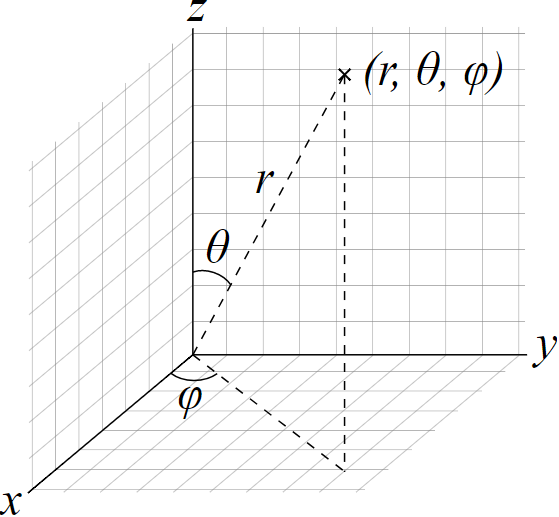
\includegraphics[keepaspectratio,scale=0.5]{Spherical_Coordinates.png}
\end{figure}

\begin{figure}[H]
	\centering
	\caption{The possible directions in secondary rays (\cite{SamplingRayDirection}).}
	\label{Secondary_Rays.}
	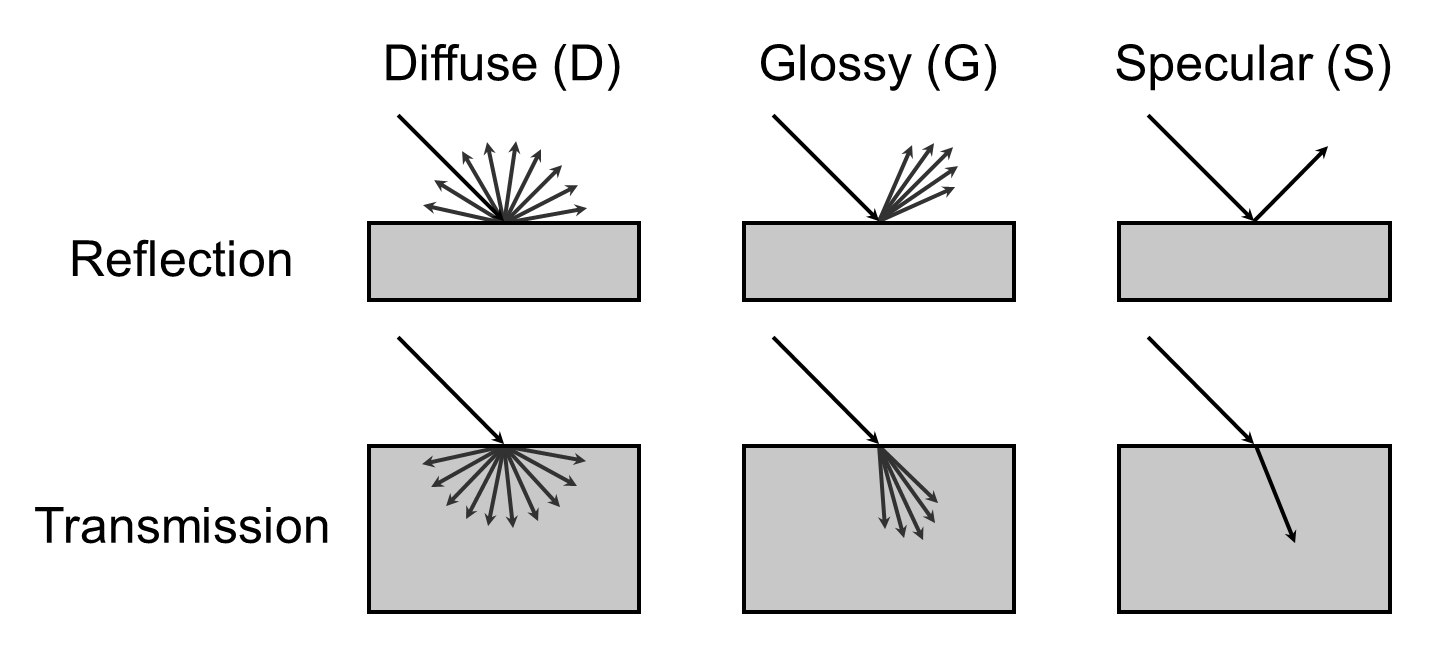
\includegraphics[keepaspectratio,scale=0.5]{SecondaryRayDirection.png}
\end{figure}

\par
The reflected and refracted light in a specular surface are simulated in a similar way to the Whitted algorithm presented previously.

\par
So, the algorithm developed in Path Tracer Shader is as following:

\begin{algorithm}
	\small
	\label{PathTracer}
	\caption{Algorithm of Path Tracer Shader}
	\Input{\var{rayDir}, \var{intersectionNormal}, \var{refractiveIndice}, \var{rayDepth}, \var{intersectionPoint}, \var{intersectionPrimitive}, \var{kD}, \var{kT}, \var{kS}}
	\Output{\var{outputRGB}}
	
	\uIf{intersected material is diffuse}{
		\ForEach{light}{
			\ForEach{sample}{
				$\var{lightPos} \gets \var{samplerLight}.getSample()$
				$\vec{vectorToLight} \gets \var{lightPos} - \var{intersectionPoint}$ \\
				$\var{cosNL} \gets \vec{vectorToLight} \cdot \vec{intersectionNormal}$ \\
				\uIf{$\var{cosNL} > 0$} {
					$\vec{shadowRay} \gets Ray(\var{intersectionPoint}, \vec{vectorToLight}, \var{distanceToLight}, \var{rayDepth} + 1)$ \\
					\uIf{$!shadowTrace(\var{shadowRay})$} {
						$\var{Ld} \gets \var{Ld} + \var{radLight} * \var{cosNL}$ \\
					}
				}
			}
		}
		$\var{Ld} \gets \var{Ld} * \var{kD}$ \\
		$\var{Ld} \gets \var{Ld} * \var{\#lights}$ \\
		$\var{Ld} \gets \var{Ld} / \var{\#samples}$ \\
		
		\uIf{\var{rayDepth} <= RAY\_DEPTH\_MIN || uniform\_dist(gen) > finish\_probability} {
			$\vec{newDir} \gets getCosineSampleHemisphere (\vec{intersectionNormal})$ \\
			$\var{secundaryRay} \gets Ray(\vec{newDir}, \var{intersectionPoint}, \var{rayDepth} + 1, \var{intersectionPrimitive})$ \\
			$\var{LiD\_RGB} \gets rayTrace(\var{secundaryRay})$ \\
			$\var{LiD} \gets \var{kD} * \var{LiD\_RGB}$ \\
			\uIf{rayDepth > RAY\_DEPTH\_MIN} {
				$\var{LiD} \gets \var{LiD} / \var{continue\_probability}$ \\
			}
			\uIf{\var{Ld} > 0} {
				$\var{LiD} \gets 0$ \\
			}
		}
	}
		
	\uIf{intersected material is specular reflective} {
		$\vec{reflectionDir} \gets glm::reflect(\vec{rayDir}, \vec{intersectionNormal})$ \\
		$\var{specularRay} \gets Ray(\vec{reflectionDir}, \var{intersectionPoint}, \var{rayDepth} + 1, \var{intersectionPrimitive})$ \\
		$\var{LiS\_RGB} \gets rayTrace(\var{specularRay})$ \\
		$\var{LiS} \gets \var{kS} * \var{LiS\_RGB}$ \\
	}
	
	\uIf{intersected material is specular refractive} {
		$\vec{refractDir} \gets glm::refract(\vec{rayDir}, \vec{intersectionNormal}, 1 / \var{refractiveIndice})$ \\
		$\var{transmissionRay} \gets Ray (\vec{refractDir}, \var{intersectionPoint}, \var{rayDepth} + 1, \var{intersectionPrimitive})$ \\
		$\var{LiT\_RGB} \gets rayTrace (\var{transmissionRay})$ \\
		$\var{LiT} \gets \var{kT} * \var{LiT\_RGB}$ \\
	}

	$\var{outputRGB} \gets \var{outputRGB} + \var{Ld} + \var{LiD} + \var{LiS} + \var{LiT}$ \\
\end{algorithm}

\begin{figure}[H]
	\centering
	\caption{PathTracer shader.}
	\label{PathTracer shader.}
	\includegraphics[keepaspectratio,scale=0.3]{PathTracer.png}
\end{figure}


\subsection{Samplers}

\par
There were implemented four samplers: Constant, Stratified, HaltonSequence and MersenneTwister.

\par
All samplers just provide one method for the user to use:

\begin{lstlisting}[caption={Main methods of Sampler}, captionpos=b, label=Sampler]
float getSample(unsigned sampleNumber);
\end{lstlisting}

\par
The
$getSample$
method receives as parameter the number of the current sample and returns the the actual sample.
An atomic variable
$sample$
is used to count the current index of the samples.

\subsubsection{Constant}

\par
This sampler is the simplest because it always returns the same number passed to the constructor.

\par
This is used when the user only needs one sample per pixel and want all the samples to be in the middle of each pixel.

\par
So, the algorithm of the
$getSample$
is just:

\begin{lstlisting}[caption={Algorithm of Constant Sampler}, captionpos=b, label=Constant]
return value
\end{lstlisting}


\subsubsection{Stratified}

\par
This sampler makes each sample at equal distance
$(1 / domainSize)$
and in ascending order.
For example, for a domain size of 4, the samples taken are going to be: 0, 0.25, 0.5 and 0.75.

\par
This is useful for taking samples when supersampling without any noise, because each sample is not randomly chosen.

\par
The algorithm of the
$getSample$
is then:

\begin{lstlisting}[caption={Algorithm of Stratified Sampler}, captionpos=b, label=Stratified]
current = sample++ //atomic operation
if (current >= (domainSize * (sampleNumber + 1))) {
  sample--
  return 1
}
unsigned task = current - (sampleNumber * domainSize)
resSample = task / domainSize
return resSample
\end{lstlisting}

\begin{algorithm}
	\small
	\label{Stratified}
	\caption{Algorithm of Stratified Sampler}
	\Input{\var{sampleNumber}}
	\Output{\var{resSample}}
	
	$\var{sample} \gets \var{sample} + 1$ //atomic operation \\
	$\var{current} \gets \var{sample}$ \\
	\eIf{current >= (domainSize * (sampleNumber + 1))}{
		$\var{sample} \gets \var{sample} - 1$ //atomic operation \\
		$\var{resSample} \gets 1$ \\
	} {
		$\var{task} \gets \var{current} - (\var{sampleNumber} * \var{domainSize})$ \\
		$\var{resSample} \gets \var{task} * \var{domainSize}$ \\
	}
\end{algorithm}

This algorithm ensures that if the current sample is greater than the domain size, then it will always return 1 which means the end of the sampler.


\subsubsection{HaltonSequence}

\par
As the name implies, this sampler generates the Halton sequence.

\par
Halton sequence is a quasi random number sequence which is a deterministic sequence with low discrepancy.
These sequences are usually good for Rendering Algorithms like Path Tracing because it can make the rendering equation converge faster, that is, with fewer samples.

\begin{figure}[H]
	\centering
	\caption{Halton sequence in a 2D image plane (\cite{HaltonSequence}).}
	\label{Halton_sequence_2D.}
	\includegraphics[keepaspectratio,scale=0.5]{Halton_sequence_2D.png}
\end{figure}

\par
The algorithm of the
$getSample$
is as following:

\begin{lstlisting}[caption={Algorithm of HaltonSequence Sampler}, captionpos=b, label=HaltonSequenceSampler]
current = sample++ //atomic operation
if (current >= (domainSize * (sampleNumber + 1))) {
  sample--
  return 1
}
unsigned task = current - (sampleNumber * domainSize)
float resSample = MobileRT::haltonSequence(task, 2)
return resSample
\end{lstlisting}

\begin{algorithm}
	\small
	\label{HaltonSequenceSampler}
	\caption{Algorithm of HaltonSequence Sampler}
	\Input{\var{sampleNumber}}
	\Output{\var{resSample}}
	
	$\var{sample} \gets \var{sample} + 1$ //atomic operation \\
	$\var{current} \gets \var{sample}$ \\
	\eIf{current >= (domainSize * (sampleNumber + 1))}{
		$\var{sample} \gets \var{sample} - 1$ //atomic operation \\
		$\var{resSample} \gets 1$ \\
	} {
		$\var{task} \gets \var{current} - (\var{sampleNumber} * \var{domainSize})$ \\
		$\var{resSample} \gets haltonSequence(\var{task}, 2)$ \\
	}
\end{algorithm}

\par
As it can be seen in listing \ref{HaltonSequenceSampler}, most of the Halton Sequence Sampler is similar to the Stratified Sampler.
The only difference is the call to the \textit{haltonSequence} method where it computes the Halton sequence for an arbitrary index and base number.

\par
The Halton sequence algorithm is very simple as shown in listing \ref{HaltonSequence} and it was taken from \cite{HaltonSequence}.

\begin{lstlisting}[caption={Developed method of HaltonSequence}, captionpos=b, label=HaltonSequence]
float haltonSequence(unsigned index, unsigned base) {
	float f = 1.0
	float result = 0.0
	while (index > 0) {
		f /= base
		result += f * (index % base)
		index = std::floor(index / base)
	}
	return result;
}
\end{lstlisting}

\begin{algorithm}
	\small
	\label{HaltonSequence}
	\caption{Developed method of HaltonSequence}
	\Input{\var{index}, \var{base}}
	\Output{\var{result}}
	
	$\var{f} \gets 1$ \\
	$\var{result} \gets 0$ \\
	\While{$\var{index} > 0$}{
		$\var{f} \gets \var{f} \div \var{base}$ \\
		$\var{result} \gets \var{result} + \var{f} \times (\var{index} \mod \var{base})$ \\
		$\var{index} \gets \floor{\var{index} \div \var{base}}$ \\
	}
\end{algorithm}

\subsubsection{MersenneTwister}

\par
This sampler is just a wrapper to call the constructor of std::uniform\_real\_distribution() and the constructor of std::random\_device() of the standard C++ library.

This allow to construct a random number generator which calculates a random number between 0 and 1 with an uniform distribution.
This generator is a pseudo random number generator (PRNG), which is an algorithm for generating a sequence of numbers whose properties approximate the properties of sequences of random numbers.
Although the PRNG-generated sequence is not truly random, because it is completely determined by an initial value, called the PRNG's seed, it commonly used a std::random\_device for the generator seed because it produces non-deterministic random numbers, when supported.
These sequences are usually used in simulations that use Monte Carlo methods like the Monte Carlo Ray Tracing.

\par
It is a good PRNG because it produces uniformly distributed numbers, it doesn't repeat the same sequence and it does not exhibit correlation between successive numbers.

\begin{figure}[H]
	\centering
	\caption{Pseudorandom sequence in a 2D image plane (\cite{HaltonSequence}).}
	\label{Pseudorandom_sequence_2D.}
	\includegraphics[keepaspectratio,scale=0.5]{Pseudorandom_sequence_2D.png}
\end{figure}

\par
So the algorithm of the
$getSample$
is just:

\begin{lstlisting}[caption={Algorithm of MersenneTwister Sampler}, captionpos=b, label=MersenneTwister]
static std::uniform_real_distribution<float> uniform_dist {0.0, 1.0}
static std::mt19937 gen(std::random_device {}())
float res = uniform_dist(gen)
return res
\end{lstlisting}

\par
As can be seen in listing \ref{MersenneTwister}, the algorithm is very simple because it just constructs two objects in the first time the method is called:

\begin{enumerate}
	\item std::uniform\_real\_distribution (paramA, paramB) - which produces random floating-point values, uniformly distributed on the interval [paramA, paramB), that the user specifies.
	\item std::mt19937 (std::random\_device {}()) - pseudo-random generator of 32-bit numbers with a state size of 19937 bits.
\end{enumerate}

\par
Then every time the user calls \textit{getSample}, the MersenneTwister Sampler just calls the operator() of std::uniform\_real\_distribution generator, which generates the next random number in the distribution.

\subsection{Lights}

\par
There were implemented two types of light sources: point light and area light.
These light sources provide the user two main methods:

\begin{lstlisting}[caption={Main methods in Light}, captionpos=b, label=Light]
glm::vec3 getPosition()
Intersection intersect(Intersection intersection, Ray ray)
\end{lstlisting}

\par
The
$getPosition$
method just returns the position of the light source and the 
$intersect$
method determines whether a given
$ray$
as a parameter intersects this light source and, if it intersects, writes the result to the
$intersection$
parameter.

\subsubsection{Point light}

\par
The Point light is the simplest form of a light because, as the name implies, it is just a point of light which emits light in all directions at once.
This type of light is useful to render fast shadows because it just simulates hard shadows, in that each shadow is only constituted with an umbra, which is the fully dark shadow.

\begin{figure}[H]
	\centering
	\caption{Hard shadows (\cite{Shadows}).}
	\label{Shadows_Hard.}
	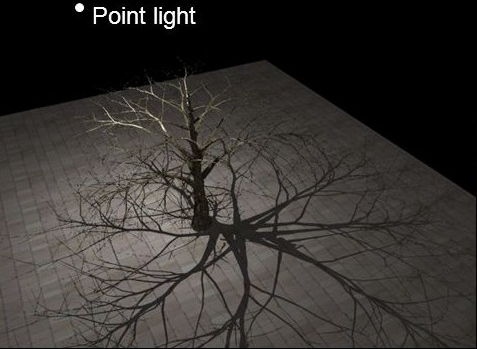
\includegraphics[keepaspectratio,scale=0.5]{Shadows_Hard.png}
\end{figure}

\par
Therefore, the
$getPosition$
method is very simple because it only returns the position of the light source determined in its constructor:

\begin{lstlisting}[caption={Algorithm of getPosition in Point light}, captionpos=b, label=getPositionPointLight]
return lightPosition
\end{lstlisting}

\par
And the
$intersect$
method is also quite simple because the ray parameter never intersects the point light.
This is because the probability of a ray intersecting a single 3D point in the world is practically null.

\begin{lstlisting}[caption={Algorithm of intersect in Point light}, captionpos=b, label=intersectPointLight]
return intersection
\end{lstlisting}

\subsubsection{Area light}

\par
The Area light is another type of light source where the light comes from an area.
It can have many different shapes, like square, triangle, circle, etc., and this allows the simulation of soft shadows like the figure \ref{Shadows_Soft.}.

\begin{figure}[H]
	\centering
	\caption{Soft shadows (\cite{Shadows}).}
	\label{Shadows_Soft.}
	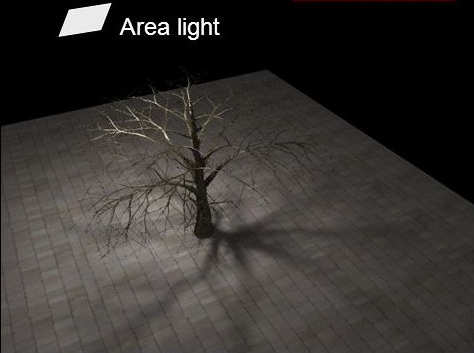
\includegraphics[keepaspectratio,scale=0.5]{Shadows_Soft.png}
\end{figure}

\par
The Area light implemented for this application has a shape of a triangle.
This shape is intended as the triangle is the simplest shape which allows to construct more complex shapes.
And, with barycentric coordinates, it is very easy to generate a random point in the triangle.

\par
A triangle with three points: A, B and C.
We get vectors AB and AC, being:

\begin{lstlisting}[caption={Vectors AB and AC in a triangle}, captionpos=b, label=AreaLight]
AB=[Bx-Ax,By-Ay,Bz-Az] and AC=[Cx-Ax,Cy-Ay,Cz-Az].
\end{lstlisting}

\par
These vectors tell us how to get from point A to the other two points in the triangle, by telling us what direction to go and how far.
So, with barycentric coordinates R=1/3, S=1/3 and T=1/3, we get the point in the center of the triangle.
To generate a random point in the triangle, we have to generate two random numbers between 0 and 1 (R and S).
Then we have to make sure we stay inside the triangle by checking if they are larger than one:

\begin{lstlisting}[caption={Algorithm of Area light}, captionpos=b, label=AreaLight]
if (R + S >= 1) {
  R = 1 - R
  S = 1 - S
}
\end{lstlisting}

Finally we can obtain a random point in the triangle by starting at point A, then getting a random percentage along vector AB and a random percentage along vector AC:

\begin{lstlisting}[caption={Algorithm of Area light}, captionpos=b, label=AreaLight]
RandomPointPosition = A + R*AB + S*AC
\end{lstlisting}

\begin{figure}[H]
	\centering
	\caption{Calculation of point P by using barycentric coordinates starting at point A and adding a vector AB and a vector AC (\cite{TriangleBarycentricCoordinates}).}
	\label{Barycentric_Coordinates.}
	\includegraphics[keepaspectratio,scale=0.5]{barycentric-coordinates.png}
\end{figure}

\par
So, the
$getPosition$
algorithm is as following:

\begin{lstlisting}[caption={Algorithm of getPosition in Area light}, captionpos=b, label=AreaLight]
float R = samplerPointLight->getSample()
float S = samplerPointLight->getSample()
if (R + S >= 1.0) {
	R = 1.0 - R;
	S = 1.0 - S;
}
glm::vec3 position = triangle.pointA + R * triangle.AB + S * triangle.AC
return position
\end{lstlisting}

\par
And the
$intersect$
method just calls the intersection of a ray with a triangle method presented earlier, and if it intersects updates the material.

\begin{lstlisting}[caption={Algorithm of intersect in Area light}, captionpos=b, label=AreaLight]
float lastDist = intersection.length
intersection = triangle.intersect(intersection, ray)
intersection.material_= intersection.length < lastDist? &radiance : intersection.material
return intersection
\end{lstlisting}

\subsection{Cameras}

\par
Only two types of cameras were implemented: perspective and orthographic cameras.

\par
The camera only provides one method for the user to cast a ray from the camera position in direction to the image plane:

\begin{lstlisting}[caption={Main methods in Camera}, captionpos=b, label=Camera]
Ray generateRay(float u, float v, float deviationU, float deviationV);
\end{lstlisting}

\par
The method
$generateRay$
needs four parameters to create a ray.
The $u$ and $v$
are used to choose the targeted pixel in the image plane.
Being
$u$
the inverse of the index of the pixel in its line, that is,
$x / width$
, and
$v$
the inverse of the index of the pixel in its column, that is,
$y / height$.
In order to allow the reduction of aliasing in the generated images of the scene, the camera also accepts two extra parameters
$deviationU$ and $deviationV$
which are variances inside a pixel.
The
$deviationU$
is a horizontal variance of the pixel, that is,\\
$[-0.5*pixelWidth, 0.5*pixelWidth]$
and
$deviationV$ the variance in the vertical of the pixel\\
$[-0.5*pixelHeight, 0.5*pixelHeight]$.
This technique is called jittering, as shown in figure \ref{Jittering.}, and allows to reduce the aliasing effect by introducing noise into the output image.
Although the final image gets some noise, this effect turns out to be visually more appealing than aliasing because it is an effect without patterns that are easily detectable by the human eye.
It is important to reduce the aliasing effect because, it is an effect that the human eyes can detect very fast because the generated image will have quite regular patterns, as shown in figure \ref{Aliased.}.

\begin{figure}[H]
	\centering
	\caption{Illustration of how sampling the plane image with jittering works (\cite{Jittering}).}
	\label{Jittering.}
	\includegraphics[keepaspectratio,scale=1.0]{Jittering.png}
\end{figure}

\begin{figure}[H]
	\centering
	\caption{Aliasing effect (\cite{Aliasing}).}
	\label{Aliased.}
	\includegraphics[keepaspectratio,scale=0.6]{aliasing.jpg}
\end{figure}


\par
Sampling with jittering is, as previously stated, a good technique to avoid aliasing in the image.
The figure \ref{Sampling_Stratified.} shows an example of stratified sampling with 1 and 256 samples per pixel.
As can be seen in the figure on the left, there is a noticeably aliasing in the image, and we can't even perceive the correct positions of the black squares on the background.
Of course, with 256 samples per pixel, the aliasing effect is greatly reduced, but also, the execution time is linearly increased, which is a downside to the user experience.

\begin{figure}[H]
	\centering
	\subfloat[Stratified sampling with 1, sample per pixel.][Stratified sampling with 1 \\sample per pixel.]{{\includegraphics[width=5cm]{regular_1spp.png} }}
	\qquad
	\subfloat[Stratified sampling with 256, samples per pixel.][Stratified sampling with 256 \\samples per pixel.]{{\includegraphics[width=5cm]{regular_256spp.png} }}
	\caption{Stratified sampling.}
	\label{Sampling_Stratified.}
\end{figure}

\par
Sampling with jittering is, obviously not perfect, as shown in the figure \ref{Sampling_Jittering.}.
But, it produces more visually appealing images, although it introduces some noise.
Even, with just 1 sample per pixel, the generated image is less "jaggy" in the background.
And, with 4 samples per pixel, the noise is greatly reduced and its quality is visually comparable to the stratified sampling with 256 samples per pixel.
This means that by using jittering it is possible to obtain images pleasing to the human eye with fewer samples per pixel, and consequently in less execution time.

\begin{figure}[H]
	\centering
	\subfloat[Jittered sampling with 1, sample per pixel.][Jittered sampling with 1 \\sample per pixel.]{{\includegraphics[width=5cm]{jittering_1spp.png} }}
	\qquad
	\subfloat[Jittered sampling with 4, samples per pixel.][Jittered sampling with 4 \\samples per pixel.]{{\includegraphics[width=5cm]{jittering_4spp.png} }}
	\caption{Jittered sampling.}
	\label{Sampling_Jittering.}
\end{figure}


\subsubsection{Perspective Camera}

\par
This type of camera is the most used in renderers because it uses perspective projection.
With it, it can simulate images being seen by the human eyes, which means, it simulates the depth of the objects, and produces 2D images with a 3D projection.

\par
To obtain an image plane with perspective, it is necessary to have a Field of View.
In order to accept any resolution of the image plane, we have to divide the field of view in two parts: horizontal and vertical.
This way, we can obtain the aspect ratio of the image plane we want.

\begin{figure}[H]
	\centering
	\caption{Perspective camera with hFov and vFov (\cite{Camera_Perspective_Orthographic}).}
	\label{Perspective_Camera.}
	\includegraphics[keepaspectratio,scale=0.6]{Camera_Perspective_v2.png}
\end{figure}

\par
The algorithm to generate a ray from the perspective camera is very simple.
By knowing the horizontal Field of View and vertical Field of View in radians, and with
$u$
and
$v$
as parameters, it is possible to calculate the direction of that ray.

\par
It starts to calculate the distance to go through the right vector and the up vector of the camera.
That can be done with the arctangent of each Field of View of the camera (horizontal and vertical) and multiplying it with
$u - 0.5$
in the right vector and with
$0.5 - v$
in the up vector.
This makes sure that we go through every pixel, starting with the pixel from the top left corner to the bottom right corner of the image plane.
Then the destination point of the ray is just the sum:\\
$destinationPoint = cameraPosition + cameraDirection + rightVector + upVector$
, and so its direction is just:\\
$rayDirection = destinationPoint - cameraPosition$
.
The origin of the ray is the position of the camera, because in a perspective camera, all rays come from the same point: the point where the camera is located.

\begin{lstlisting}[caption={Algorithm of generateRay in Perspective Camera}, captionpos=b, label=Perspective]
float rightFactor = arctan(hFov * (u - 0.5)) + deviationU
glm::vec3 rightVector = right * rightFactor
float upFactor = arctan(vFov * (0.5 - v)) + deviationV
glm::vec3 upVector = up * upFactor
glm::vec3 destinationPoint = cameraPosition + cameraDirection + rightVector + upVector
glm::vec3 rayDirection = destinationPoint - cameraPosition
Ray ray = Ray(glm::normalize(rayDirection), cameraPosition)
return ray
\end{lstlisting}


\subsubsection{Orthographic Camera}

\par
In this projection mode, an object's size in the rendered image stays constant regardless of its distance from the camera.
This can be useful for rendering 2D scenes and UI elements, amongst other things.

\par
The orthographic camera removes the sense of perspective by drawing the image plane without simulating the depth of the objects, making all the objects looking flat.
This is achieved by inverting the logic of the perspective camera.
Instead of calculating the direction and always having the same origin, in the orthographic camera, the direction is always the same for all rays, and the origin of the ray varies.

\par
It starts to calculate the distance to go through the right vector and up vector of the camera, like the perspective camera.
But, instead of using the Field of View, we now use the
$sizeH$
and
$sizeV$
, which are the horizontal and vertical sizes of the image plane.
Then, to make sure that we go through all pixels from top left pixel to the bottom right, we need to use the
$u$
and
$v$
values from the parameters.
Then, the origin of the ray is:
$rayOrigin = cameraPosition + rightVector + upVector$
.

\begin{lstlisting}[caption={Algorithm of generateRay in Orthographic Camera}, captionpos=b, label=Orthographic]
float rightFactor = (u - 0.5) * sizeH
glm::vec3 rightVector = right * rightFactor + right * deviationU
float upFactor = (0.5 - v) * sizeV
glm::vec3 upVector = up * upFactor + up * deviationV
glm::vec3 rayOrigin = cameraPosition + rightVector + upVector
Ray ray = Ray (cameraDirection, rayOrigin)
return ray
\end{lstlisting}

\begin{figure}[H]
	\centering
	\caption{Orthographic camera with sizeH and sizeV (\cite{Camera_Perspective_Orthographic}).}
	\label{Perspective_Camera.}
	\includegraphics[keepaspectratio,scale=0.6]{Camera_Orthographic_v2.png}
\end{figure}


\subsection{Object Loaders}

\par
Last, but not least, the library allows the programmer to develop his / her own Object Loaders.
An Object Loader is, as the name implies, a class that allows the ray tracer to import meshes from different Model file formats.
There are many different types of file formats for storing meshes:

\begin{itemize}
	\item 3ds
	\item FBX
	\item Wavefront .obj file
	\item COLLADA
	\item SketchUp
	\item AutoCAD DXF
\end{itemize}

\par
All these file formats allows the user to store the positions of many triangles in a file, which together form the geometry of the scene.

\par
This library only provides one Object Loader that allows loading the scene geometry from Wavefront obj files, which was achieved using a third party library called "tinyobjloader".
This type of Model file format is a good choice because, besides being simple, it is open and has been adopted by many 3D graphics application vendors, like, 3ds Max and Blender.

\subsubsection{OBJ Loader}

\par
The class "OBJLoader" is a Rendering Component that allows the user to load 3D scenes from Wavefront obj files.

\par
The OBJ file format is a simple file data format that allows to store only the position of each vertex, the UV position of each texture coordinate vertex, each vertex normal, and the faces that make each polygon defined as a list of vertices, and texture vertices.
Vertices are stored in a counter-clockwise order by default, making explicit declaration of face normals unnecessary.

\begin{lstlisting}[caption={.OBJ file format}, captionpos=b, label=OBJ]
	# This is a comment

	# List of geometric vertices
	# x   y   z   w
	v 1.0 2.0 3.0 1.0
	v 5.0 6.0 7.0 1.0
	...
	
	# List of texture coordinates
	#  x   y   w
	vt 0.5 1.0 0.0
	vt 0.1 0.3 0.0
	...
	
	# List of vertices normals
	#  x   y   z
	vn 0.3 0.0 0.7
	vn 0.2 1.0 0.3
	...
	
	# List of polygonal face elements
	# v1/vt1/vn1	v2/vt2/vn2	v3/vt3/vn3
	f 03/01/01			04/02/03		05/03/04
	f 06/06/03			07/01/02		08/02/06
	...
\end{lstlisting}

\par
The Wavefront OBJ file format is described as shown in \ref{OBJ}, and is accompanied by another file, Material Template Library (MTL), that describes the visual aspects of the polygons.
It is this file that describes surface shading (material) properties of objects within one or more .OBJ files.
It allows to define multiple materials, with, ambient color, diffuse color, specular reflective color and specular refractive color.
And even allows to load texture maps stored in TGA files.
The listing \ref{MTL} shows an example of a description of a material.

\begin{lstlisting}[caption={.MTL file format}, captionpos=b, label=MTL]
# This is a comment

# Define a material named 'Colored'
newmtl Colored

# Ambient color
Ka 1.0 0.0 0.0	# red

# Diffuse color
Kd 0.0 1.0 0.0	# green

# Specular color
Ks 0.0 0.0 1.0	# blue

# Dissolved (transparency)
d 0.4
\end{lstlisting}

% Chapter - Android
% CHAPTER - falar de como uma aplicaçao android funciona
% CHAPTER - falar de como se liga codigo C++ nativo com Java interface
% CHAPTER - falar de cuidados que tive na implementaçao para android
% CHAPTER - falar das possibilidades do android
% CHAPTER - falar das desvantagens do android
\chapter{Android challenges}

\section{Android specifics}

\par
Before developing the ray tracer to Android, it is necessary to understand how an Android application works.

\par
A typical Android application is programmed in Java programming language.
And it usually needs to communicate with an User Interface which also is programmed in Java.
The code is compiled with Android Software Development Kit (SDK) along with any data and resource files into an Android package (APK).
But, in order to avoid using the Java Virtual Machine (JVM) in our code and program it in native code, it is necessary to use Android Native Development Kit (NDK).
Unfortunately, the NDK tool-chain doesn't provide any User Interface libraries like Qt, GTKmm, or wxWidgets, that facilitates the build of a User Interface in native code.
So, in order to obtain the best performance possible in a mobile device, the ray tracer library and components were programmed in C++ and the User Interface was programmed in Java.
The User Interface calls the ray tracer available methods using the Java Native Interface (JNI) which is a programming standard that allows Java code running on a JVM to call native applications (programs specific to a hardware platform and operating system) and libraries written in other languages such as C, C ++ and assembly.
The use of JNI to call native applications is not guaranteed to have better performance than having all the application written in Java, because each JNI call have a performance cost associated with the fact that the JVM needs to use call external native code.
But, in this case as the ray tracer can be a very computing demanding application, the fact it is written in native code (C++) is better than having all the code written in Java and executed by the JVM.

\begin{figure}[H]
	\centering
	\caption{Diagram explaining how the JVM can call native code (\cite{JNI}).}
	\label{JNI.}
	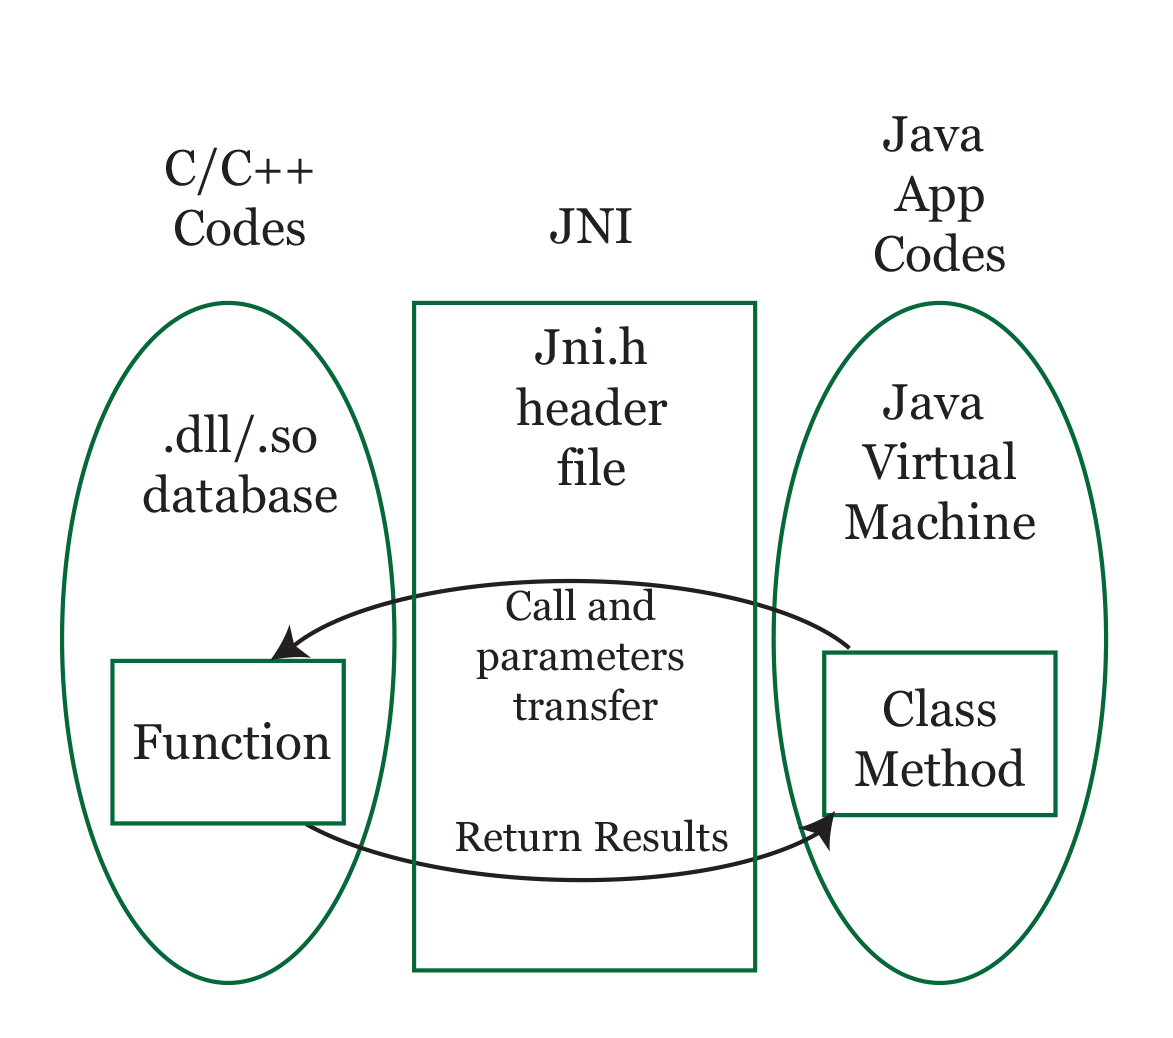
\includegraphics[keepaspectratio,scale=0.3]{JNI.png}
\end{figure}


\section{User Interface}

\par
The Android User Interface is programmed in Java and only one thread can refresh the User Interface (UI thread).

\par
There are only two goals in the User Interface: should be as simple as possible and should be able to allow progressive ray tracing, which means, refreshing the image while it is being rendered.

\par
In order to allow progressive ray tracing, it was used a pool of one thread called Render Task thread that every 250 ms wakes up the thread and updates the strings used in the text view.
Before it finishes, it publishes the progress on the UI thread.
Then the UI thread wakes up and updates the text view.

\begin{figure}[H]
	\centering
	\caption{Execution flow of UI thread and Render Task thread.}
	\label{Execution flow of UI thread and Render Task thread}
	\includegraphics[keepaspectratio,scale=0.5]{UI_thread.png}
\end{figure}

\section{Programming decisions}

\par
The main goal of programming this library in a object oriented manner is to have a library with relatively good performance and with a maintainable code.

\par
Besides that, it was used the smart pointers available in the C++ standard library.
The smart pointer used was the unique pointer, as this was enough for this project and also because it is the smart pointer with best performance.
This smart pointer automatically free the resources it contains.
This greatly reduces the chance of the programmer to forget to free a resource or trying to free it multiple times.
Of course this comes with a little performance cost of about 1\% to 5\% relatively to the manual resource management by the programmer.
But for this project, some extra code correctness is more important than more performance.

\subsection{Android benefits}

\par
As mentioned above, this dissertation focuses only on ray tracing in Android.
This is intentional because, as also mentioned above, it is the Operating System for mobile devices with the most market share.

\par
Developing apps in Android it’s cheaper than in other platforms.
The company provides its SDK for free, so all the costs are destinated to the app testing and deploying.
That means you don’t have to make a big investment in that part.
Investing less on your app development means that you’ll have a higher ROI and your project will be more profitable.

\par
Software developers, commonly learn to develop in Java, and it is easier for them to adapt to that programming language for mobile app development.
Android is built mostly in Java, so its adaptation becomes faster and easier.

\subsection{Android challenges}

\par
Developing applications for mobile devices have different challenges compared with the traditional personal computer hardware.

\par
The Android User Interface has some particularities like only one thread can modify the UI, and is usually called the UI thread.

\par
The size of RAM available for executing applications is typically smaller.
In the 2010s the most expensive mobile devices had only about 512MB of RAM, and nowadays most of them have more than 4GB.
But, still, comparing them with personal computers which typically have 16GB it is a big difference.
This can make a big impact in the maximum number of vertices that a scene can have in the ray tracer.

\par
And the CPU microarchitecture is generally simpler and with smaller computational power.
Also the Operating System (OS) is shaped for the mobile world, making a lot of restrictions in the performance of the applications in order to save battery.
The amount of main memory available for the applications can also be affected by the OS.

\par
Other challenges are related with the communication mechanism between the SDK and the NDK, because two different languages environments need to "communicate" in runtime (GUI in Java and the library in C++).
This involves learning how to use the Java Native Interface (JNI), so that the native code can send and receive information from Java Virtual Machine (JVM).

\par
Because ray tracing may involve rendering complex scenes, placing all this information in the main memory may not be possible, and so this memory management can be a worthy challenge.

% Chapter - Demonstration -------------------------
% CHAPTER - falar dos resultados obtidos
\chapter{Demonstration: Global Illumination}

\section{Results obtained}
\label{ResultsObtained}

\par
The developed application was tested in three different devices:

\begin{itemize}
	\item Samsung Galaxy Fresh Duos GT-S7392
	\item Raspberry Pi 2 Model B
	\item MINIX NEO X8-H PLUS (k200)
\end{itemize}

\begin{table}[H]
	\small
	\centering
	\caption{Devices specifications.}
	\label{specs}
	\hspace*{-2cm}
	\begin{tabular}{|l|l|l|l|l|}
		\hline
		Device&CPU&Cache(L1/L2/L3)&GPU&RAM\\ \hline
		Samsung Galaxy Fresh&1xARM Cortex A9 @1GHz&64KB/Unknown&1xBroadcom VideoCore IV&512MB\\ \hline
		Raspberry Pi 2 Model B&4xARM Cortex A7 @900MHz&64KB/1MB&1xBroadcom VideoCore IV&1GB\\ \hline
		MINIX NEO X8 PLUS&4xARM Cortex A9r4 @2.0GHz&64KB/Unknown&8xMali-450&2GB\\ \hline
	\end{tabular}
\end{table}

\par
As you can see in the table \ref{specs}, the application has been tested on a few devices.
Unfortunately, it was only possible to test it on one mobile device, the Samsung Galaxy Fresh Duos GT-S7392.
This device is a low-end smartphone with a low-end single core CPU.

\par
It was also possible to test it on two different computers that are portable and even smaller than a common laptop.
The Raspberry Pi 2 Model B and the MINIX NEO X8-H PLUS which are devices with the Android operating system installed.

\par
In order to assess the performance of the ray tracer, it was tested with three different scenes and with Whitted and Path Tracing shaders.
One large scene with some hundred of thousands triangles, one moderate with few thousand of triangles and one small scene with just some dozens triangles.

\par
The large scene used for testing was the conference scene, as illustrated in figure \ref{scene_conference}.
This scene consists of 331179 triangles and has two area lights in form of triangles.

\begin{figure}[H]
	\centering
	\caption{Illustration of conference scene, rendered with shader Whitted in MobileRT.}
	\label{scene_conference}
	\includegraphics[keepaspectratio,scale=0.5]{Scene_Conference.png}
\end{figure}

The medium scene used for testing was the Porsche 911 GT2 scene, as illustrated in figure \ref{scene_porsche}.
This scene consists of 22017 triangles and has two area lights in form of triangles.

\begin{figure}[H]
	\centering
	\caption{Illustration of Porsche 911 GT2 scene, rendered with shader Whitted in MobileRT.}
	\label{scene_porsche}
	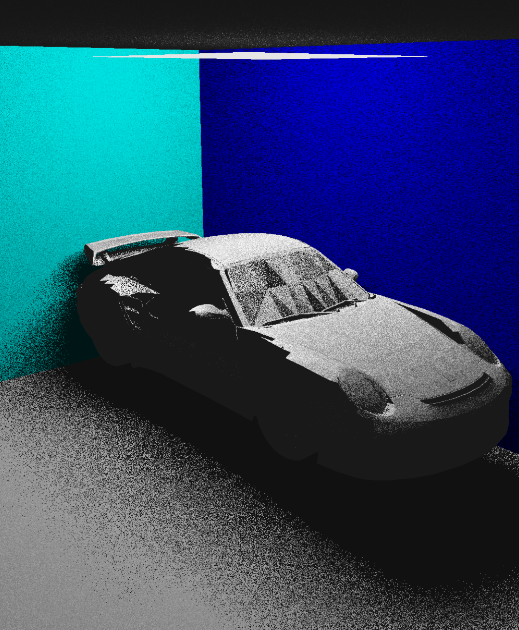
\includegraphics[keepaspectratio,scale=0.5]{Scene_Porsche.png}
\end{figure}

The small scene used for testing was the Cornell Box scene, as illustrated in figure \ref{scene_cornellbox}.
This scene consists of 34 triangles and has two area lights in form of triangles.

\begin{figure}[H]
	\centering
	\caption{Illustration of Cornell Box scene, rendered with shader Whitted in MobileRT.}
	\label{scene_cornellbox}
	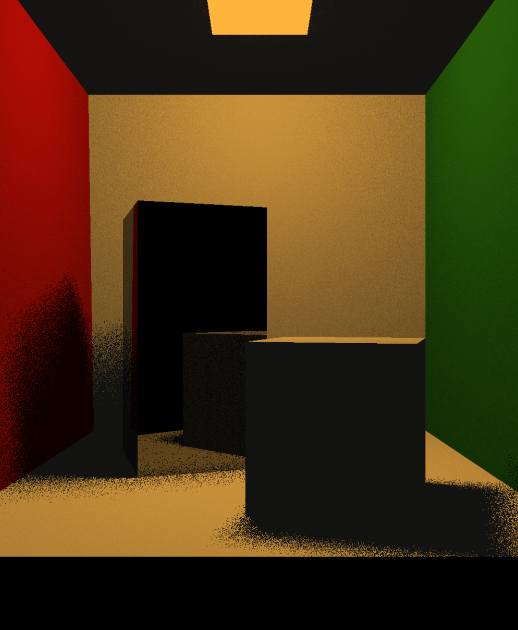
\includegraphics[keepaspectratio,scale=0.5]{Scene_CornellBox.png}
\end{figure}

\par
All of the used scenes models were downloaded from
\url{http://casual-effects.com/data/index.html}  (\cite{McGuire2017Data}).

\subsection{Whitted Shader}

\subsubsection{Samsung Galaxy Fresh Duos GT-S7392}

\begin{figure}[H]
	\begin{tikzpicture}
	\begin{semilogyaxis}[
	legend style={at={(1.05,1.00)},anchor=north west},
	xlabel = \#threads,
	ylabel = time (s),
	xtick={1,2,3,4},
	ytick={156.68,687.74,500000},
	yticklabels={156.68,687.74,500000},
	extra y ticks = 0,
	extra y tick labels = 0,
	ymin=0,
	ymax=500000,
	width=0.75\textwidth,
	]
	\addplot [
	color=blue,
	mark=*,
	dashed,
	] plot coordinates {
		(0,0.0)
		(1,500000)
	};
	\addlegendentry{Naive}
	\addplot [
	color=black,
	mark=*,
	dashed,
	] plot coordinates {
		(0,0.0)
		(1,687.74)
	};
	\addlegendentry{Regular Grid}
	\addplot [
	color=red,
	mark=*,
	dashed,
	] plot coordinates {
		(0,0.0)
		(1,156.68)
	};
	\addlegendentry{BVH}
	\label{graph:SamsungTime}
	\end{semilogyaxis}
	\end{tikzpicture}
	\caption{Time in the Conference scene}
\end{figure}

\begin{figure}[H]
	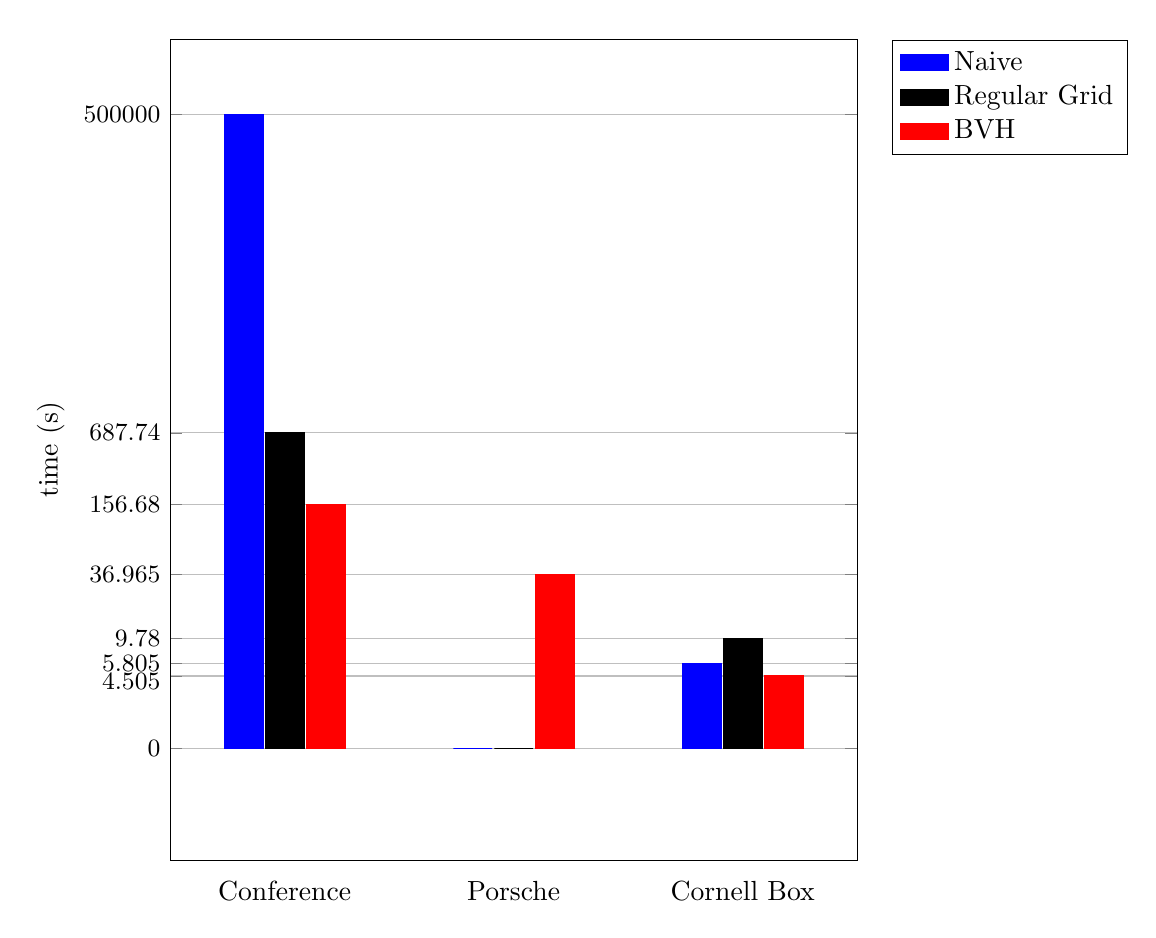
\begin{tikzpicture}
	\begin{axis}[
	legend style={at={(1.05,1.00)},anchor=north west},
	ylabel near ticks,
	ylabel = time (s),
	symbolic x coords={Conference, Porsche, Cornell Box},
	xtick=data,
	ytick={1,156.68,687.74,500000,36.965,5.805,9.78,4.505},
	yticklabels={0,156.68,687.74,500000,36.965,5.805,9.78,\smash{\raisebox{-5pt}{4.505}}},
	scaled ticks=false,
	ymode = log,
	xmode = linear,
	yticklabel style={
		font=\small,
		%/pgf/number format/.cd,
		%fixed,
		%precision=0,
		%/pgf/number format/fixed zerofill,
	},
	width  = 0.85*\textwidth,
	height = 12cm,
	major x tick style = transparent,
	ybar=2*\pgflinewidth,
	bar width=14pt,
	ymajorgrids = true,
	enlarge x limits=0.25,
	ymin=0.1,
	legend cell align=left,
	]
	\addplot[ybar,fill=blue,color=blue,area legend] coordinates {
		(Conference,   0)
		(Conference,   500000)
		(Porsche,  	1)
		(Cornell Box,   5.805)
	};
	\addlegendentry{Naive}

	\addplot[ybar,fill=black,color=black,area legend] coordinates {
		(Conference,   0)
		(Conference,   687.74)
		(Porsche,  	1)
		(Cornell Box,   9.78)
	};
	\addlegendentry{Regular Grid}
	
		\addplot[ybar,fill=red,color=red,area legend] coordinates {
		(Conference,   0)
		(Conference,   156.68)
		(Porsche,  	36.965)
		(Cornell Box,   4.505)
	};
	\addlegendentry{BVH}
	
	\end{axis}
	\label{graph:SamsungTime2}
	\end{tikzpicture}
	\caption{Time with Samsung smartphone}
\end{figure}

\begin{table}[H]
	\begin{tabular}{|l|l|l|l|l|}
		\hline
		Scene & Accelerator & \#Threads & Time (s) & Speedup \\ \hline
		Conference & Naive & 1 & X & 1 \\ \hline
		Conference & Reg Grid & 1 & 687.74 & 727 \\ \hline
		Conference & BVH & 1 & 156.68 & 3191 \\ \hline
		Porsche & Naive & 1 & 14 & 1 \\ \hline
		Porsche & Reg Grid & 1 & 14 & 15 \\ \hline
		Porsche & BVH & 1 & 36.965 & 15 \\ \hline
		Cornell Box & Naive & 1 & 5.805 & 1 \\ \hline
		Cornell Box & Reg Grid & 1 & 9.78 & 0.59 \\ \hline
		Cornell Box & BVH & 1 & 4.505 & 1.29 \\ \hline
	\end{tabular}
\end{table}

\begin{figure}[H]
	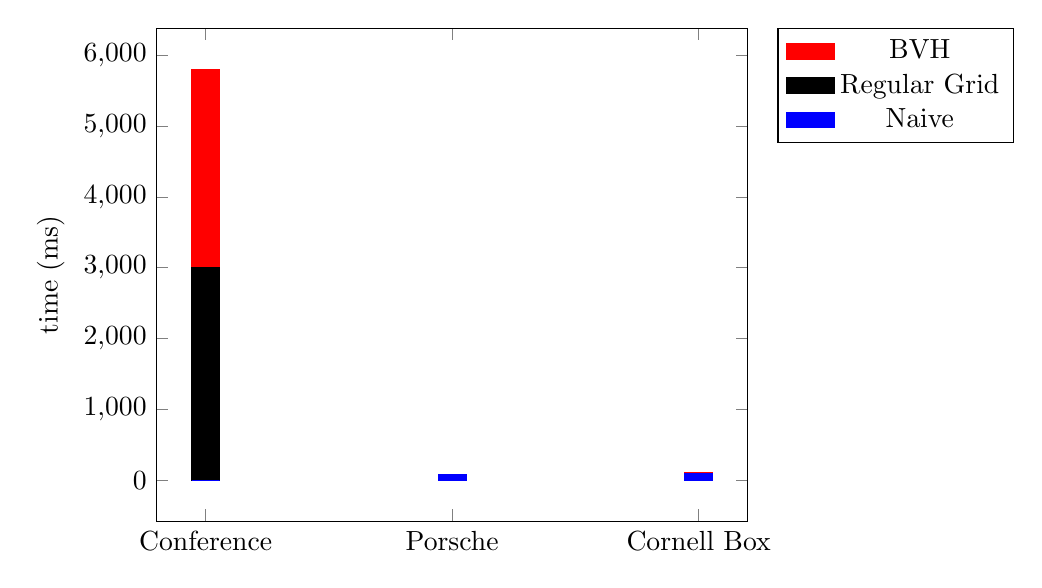
\begin{tikzpicture}
	\begin{axis}[
	legend style={at={(1.05,1.00)},anchor=north west},
	ylabel = time (ms),
	symbolic x coords={Conference, Porsche, Cornell Box},
	xtick=data,
	width=0.75\textwidth,
	scaled ticks=false,
	yticklabel style={
		/pgf/number format/.cd,
		fixed,
		precision=0,
		/pgf/number format/fixed zerofill,
	}
	]
	\addplot[ybar,fill=red,color=red,area legend] coordinates {
		(Conference,   0)
		(Conference,   5800)
		(Porsche,  	85)
		(Cornell Box,   105)
	};
	\addlegendentry{BVH}
	\addplot[ybar,fill=black,color=black,area legend] coordinates {
		(Conference,   0)
		(Conference,   3000)
		(Porsche,  	80)
		(Cornell Box,   99)
	};
	\addlegendentry{Regular Grid}
	\addplot[ybar,fill=blue,color=blue,area legend] coordinates {
		(Conference,   0)
		(Conference,   0)
		(Porsche,  	77)
		(Cornell Box,   91)
	};
	\addlegendentry{Naive}
	\end{axis}
	\label{graph:SamsungConstruct}
	\end{tikzpicture}
	\caption{Time to construct accelerators in Samsung Galaxy smart phone}
\end{figure}

\begin{figure}[H]
	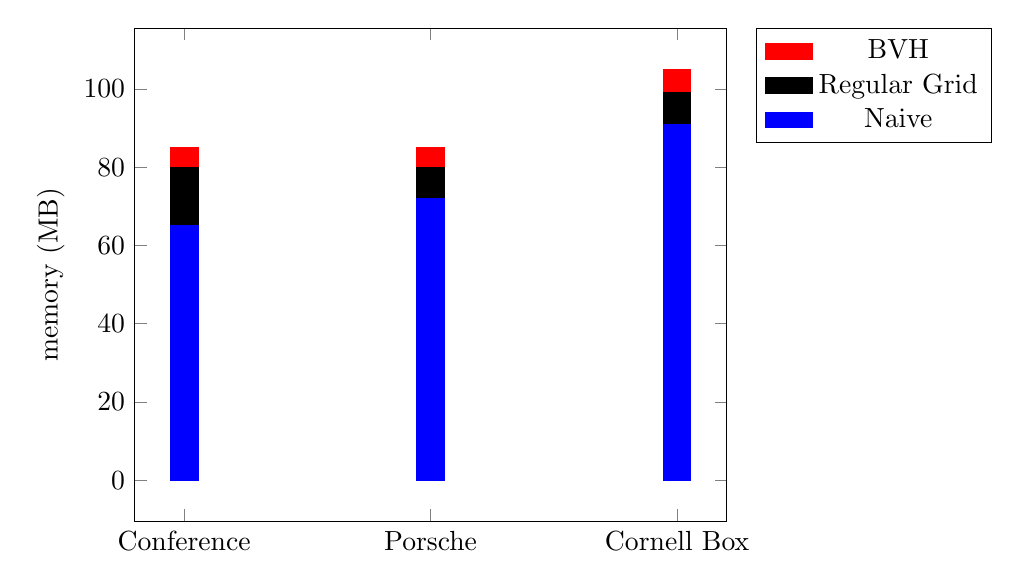
\begin{tikzpicture}
	\begin{axis}[
	legend style={at={(1.05,1.00)},anchor=north west},
	ylabel = memory (MB),
	symbolic x coords={Conference, Porsche, Cornell Box},
	xtick=data,
	width=0.75\textwidth,
	]
	\addplot[ybar,fill=red,color=red,area legend] coordinates {
		(Conference,   0)
		(Conference,   85)
		(Porsche,  	85)
		(Cornell Box,   105)
	};
	\addlegendentry{BVH}
	\addplot[ybar,fill=black,color=black,area legend] coordinates {
		(Conference,   0)
		(Conference,   80)
		(Porsche,  	80)
		(Cornell Box,   99)
	};
	\addlegendentry{Regular Grid}
	\addplot[ybar,fill=blue,color=blue,area legend] coordinates {
		(Conference,   0)
		(Conference,   65)
		(Porsche,  	72)
		(Cornell Box,   91)
	};
	\addlegendentry{Naive}
	\end{axis}
	\label{graph:SamsungMemory}
	\end{tikzpicture}
	\caption{Memory usage in the Samsung Galaxy smart phone}
\end{figure}

\subsubsection{Raspberry Pi 2 Model B}

\begin{figure}[H]
	\begin{tikzpicture}
	\begin{axis}[
	legend style={at={(1.05,1.00)},anchor=north west},
	axis lines = left,
	xlabel = \#threads,
	ylabel = time (ms),
	xtick={0,1,2,3,4},
	ytick={0,1,...,10},
	width=0.75\textwidth,
	]
	\addplot [
	color=blue,
	mark=*,
	dashed,
	] plot coordinates {
		(0,0.0)
		(1,1.0)
		(2,1.0)
		(3,1.0)
		(4,1.0)
	};
	\addlegendentry{Naive}
	\addplot [
	color=black,
	mark=*,
	dashed,
	] plot coordinates {
		(0,0.0)
		(1,1.0)
		(2,1.0)
		(3,1.0)
		(4,1.0)
	};
	\addlegendentry{Regular Grid}
	\addplot [
	color=red,
	mark=*,
	dashed,
	] plot coordinates {
		(0,0.0)
		(1,1.0)
		(2,1.0)
		(3,1.0)
		(4,1.0)
	};
	\addlegendentry{BVH}
	\label{graph:RaspberryTime}
	\end{axis}
	\end{tikzpicture}
\end{figure}

\begin{figure}[H]
	\begin{tikzpicture}
	\begin{axis}[
	legend style={at={(1.05,1.00)},anchor=north west},
	axis lines = left,
	xlabel = \#threads,
	ylabel = speedup,
	xtick={0,1,2,3,4},
	ytick={0,1,...,10},
	width=0.75\textwidth,
	]
	\addplot [
	color=blue,
	mark=*,
	dashed,
	] plot coordinates {
		(0,0.0)
		(1,1.0)
		(2,1.0)
		(3,1.0)
		(4,1.0)
	};
	\addlegendentry{Naive}
	\addplot [
	color=black,
	mark=*,
	dashed,
	] plot coordinates {
		(0,0.0)
		(1,1.0)
		(2,1.0)
		(3,1.0)
		(4,1.0)
	};
	\addlegendentry{Regular Grid}
	\addplot [
	color=red,
	mark=*,
	dashed,
	] plot coordinates {
		(0,0.0)
		(1,1.0)
		(2,1.0)
		(3,1.0)
		(4,1.0)
	};
	\addlegendentry{BVH}
	\label{graph:RaspberrySpeedup}
	\end{axis}
	\end{tikzpicture}
\end{figure}

\begin{figure}[H]
	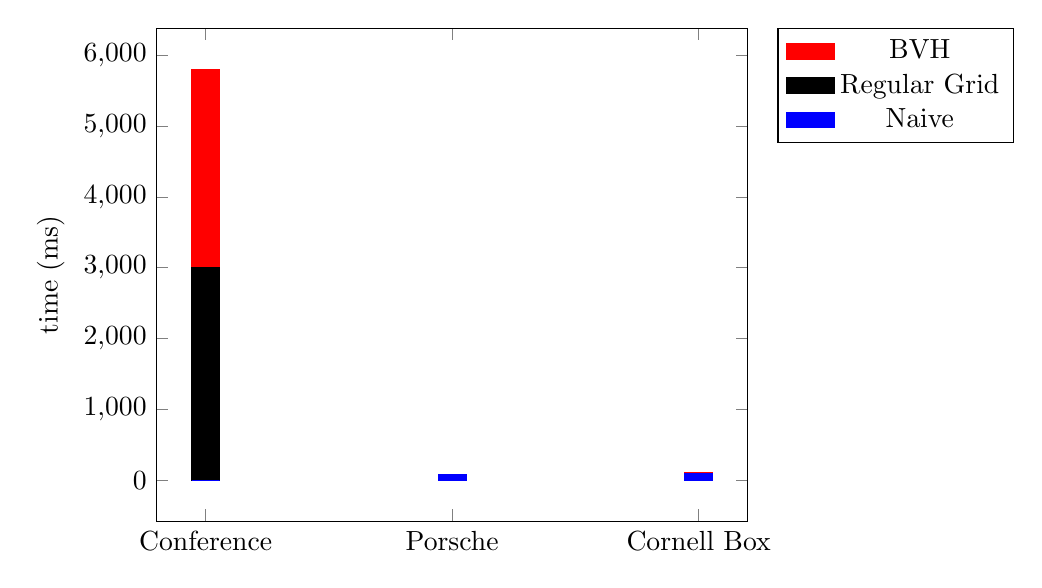
\begin{tikzpicture}
	\begin{axis}[
	legend style={at={(1.05,1.00)},anchor=north west},
	ylabel = time (ms),
	symbolic x coords={Conference, Porsche, Cornell Box},
	xtick=data,
	width=0.75\textwidth,
	]
	\addplot[ybar,fill=red,color=red,area legend] coordinates {
		(Conference,   0)
		(Conference,   5800)
		(Porsche,  	85)
		(Cornell Box,   105)
	};
	\addlegendentry{BVH}
	\addplot[ybar,fill=black,color=black,area legend] coordinates {
		(Conference,   0)
		(Conference,   3000)
		(Porsche,  	80)
		(Cornell Box,   99)
	};
	\addlegendentry{Regular Grid}
	\addplot[ybar,fill=blue,color=blue,area legend] coordinates {
		(Conference,   0)
		(Conference,   0)
		(Porsche,  	77)
		(Cornell Box,   91)
	};
	\addlegendentry{Naive}
	\end{axis}
	\label{graph:RaspberryConstruct}
	\end{tikzpicture}
	\caption{Time to construct accelerators in the Raspberry Pi 2 Model B}
\end{figure}

\begin{figure}[H]
	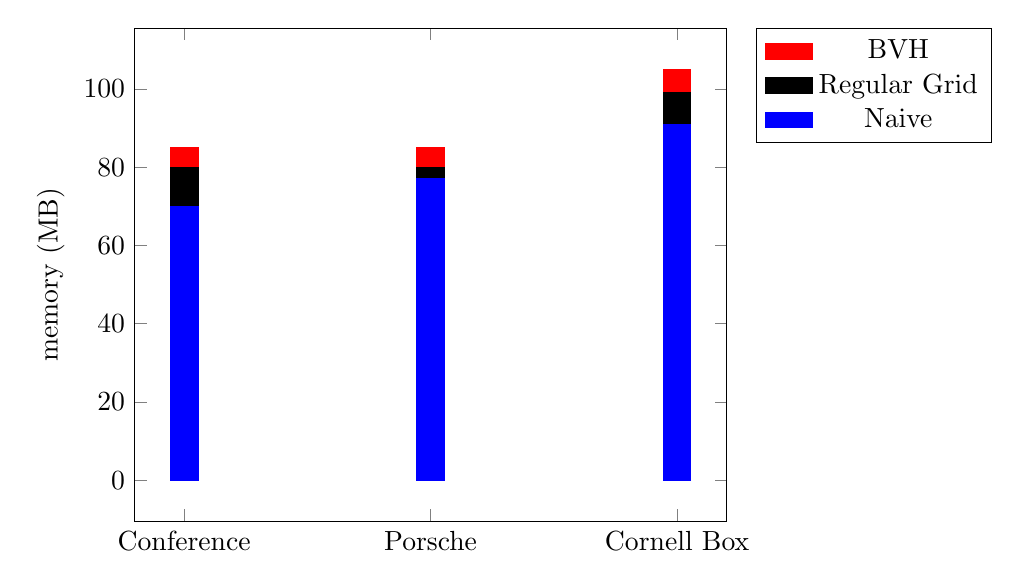
\begin{tikzpicture}
	\begin{axis}[
	legend style={at={(1.05,1.00)},anchor=north west},
	ylabel = memory (MB),
	symbolic x coords={Conference, Porsche, Cornell Box},
	xtick=data,
	width=0.75\textwidth,
	]
	\addplot[ybar,fill=red,color=red,area legend] coordinates {
		(Conference,   0)
		(Conference,   85)
		(Porsche,  	85)
		(Cornell Box,   105)
	};
	\addlegendentry{BVH}
	\addplot[ybar,fill=black,color=black,area legend] coordinates {
		(Conference,   0)
		(Conference,   80)
		(Porsche,  	80)
		(Cornell Box,   99)
	};
	\addlegendentry{Regular Grid}
	\addplot[ybar,fill=blue,color=blue,area legend] coordinates {
		(Conference,   0)
		(Conference,   70)
		(Porsche,  	77)
		(Cornell Box,   91)
	};
	\addlegendentry{Naive}
	\end{axis}
	\label{graph:RaspberryMemory}
	\end{tikzpicture}
	\caption{Memory usage in the Raspberry Pi 2 Model B}
\end{figure}


\subsubsection{MINIX NEO X8-H PLUS}

\begin{figure}[H]
	\begin{tikzpicture}
	\begin{axis}[
	legend style={at={(1.05,1.00)},anchor=north west},
	axis lines = left,
	xlabel = \#threads,
	ylabel = time (ms),
	xtick={0,1,2,3,4},
	ytick={0,533,586,760,1300},
	width=0.75\textwidth,
	]
	\addplot [
	color=blue,
	mark=*,
	dashed,
	] plot coordinates {
		(0,0.0)
		(1,1.0)
		(2,1.0)
		(3,1.0)
		(4,1.0)
	};
	\addlegendentry{Naive}
	\addplot [
	color=black,
	mark=*,
	dashed,
	] plot coordinates {
		(0,0.0)
		(1,1348.24)
		(2,760.105)
		(3,586)
		(4,533.495)
	};
	\addlegendentry{Regular Grid}
	\addplot [
	color=red,
	mark=*,
	dashed,
	] plot coordinates {
		(0,0.0)
		(1,375.945)
		(2,188.99)
		(3,125.425)
		(4,97.885)
	};
	\addlegendentry{BVH}
	\label{graph:MinixTime}
	\end{axis}
	\end{tikzpicture}
	\caption{Time in the Conference scene}
\end{figure}

\begin{figure}[H]
	\begin{tikzpicture}
	\begin{axis}[
	legend style={at={(1.05,1.00)},anchor=north west},
	axis lines = left,
	xlabel = \#threads,
	ylabel = speedup,
	xtick={0,1,2,3,4},
	ytick={0,1,...,10},
	width=0.75\textwidth,
	]
	\addplot [
	color=blue,
	mark=*,
	dashed,
	] plot coordinates {
		(0,0.0)
		(1,1.0)
		(2,1.0)
		(3,1.0)
		(4,1.0)
	};
	\addlegendentry{Naive}
	\addplot [
	color=black,
	mark=*,
	dashed,
	] plot coordinates {
		(0,0.0)
		(1,1.0)
		(2,1.0)
		(3,1.0)
		(4,1.0)
	};
	\addlegendentry{Regular Grid}
	\addplot [
	color=red,
	mark=*,
	dashed,
	] plot coordinates {
		(0,0.0)
		(1,1.0)
		(2,1.0)
		(3,1.0)
		(4,1.0)
	};
	\addlegendentry{BVH}
	\label{graph:MinixSpeedup}
	\end{axis}
	\end{tikzpicture}
\end{figure}

\begin{figure}[H]
	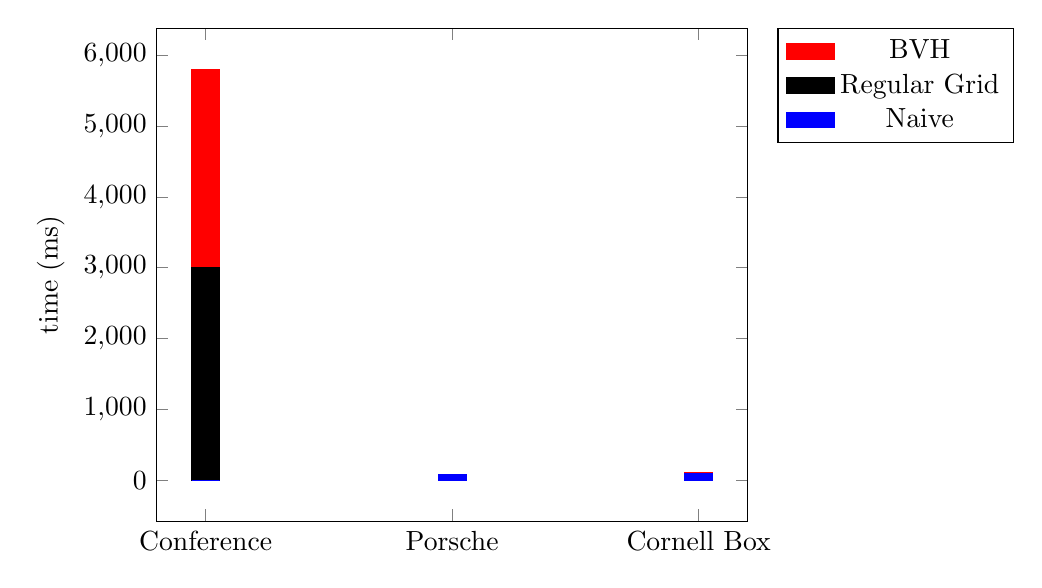
\begin{tikzpicture}
	\begin{axis}[
	legend style={at={(1.05,1.00)},anchor=north west},
	ylabel = time (ms),
	symbolic x coords={Conference, Porsche, Cornell Box},
	xtick=data,
	width=0.75\textwidth,
	]
	\addplot[ybar,fill=red,color=red,area legend] coordinates {
		(Conference,   0)
		(Conference,   5800)
		(Porsche,  	85)
		(Cornell Box,   105)
	};
	\addlegendentry{BVH}
	\addplot[ybar,fill=black,color=black,area legend] coordinates {
		(Conference,   0)
		(Conference,   3000)
		(Porsche,  	80)
		(Cornell Box,   99)
	};
	\addlegendentry{Regular Grid}
		\addplot[ybar,fill=blue,color=blue,area legend] coordinates {
		(Conference,   0)
		(Conference,   0)
		(Porsche,  	77)
		(Cornell Box,   91)
	};
	\addlegendentry{Naive}
	\end{axis}
	\label{graph:MinixConstruct}
	\end{tikzpicture}
	\caption{Time to construct accelerators in the MINIX NEO X8-H PLUS}
\end{figure}

\begin{figure}[H]
	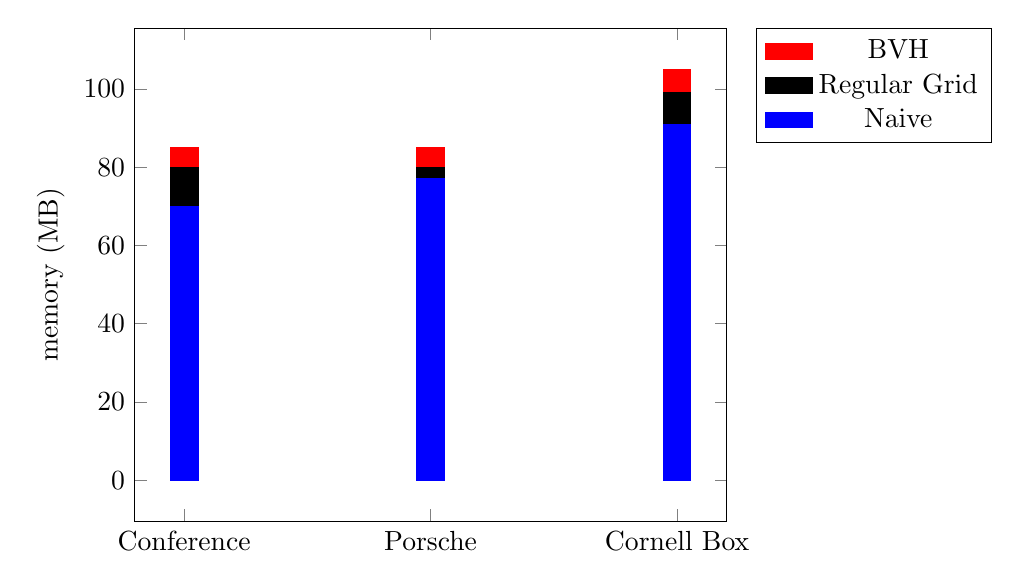
\begin{tikzpicture}
	\begin{axis}[
	legend style={at={(1.05,1.00)},anchor=north west},
	ylabel = memory (MB),
	symbolic x coords={Conference, Porsche, Cornell Box},
	xtick=data,
	width=0.75\textwidth,
	]
	\addplot[ybar,fill=red,color=red,area legend,width=4.30\textwidth] coordinates {
		(Conference,   0)
		(Conference,   85)
		(Porsche,  	85)
		(Cornell Box,   105)
	};
	\addlegendentry{BVH}
	\addplot[ybar,fill=black,color=black,area legend] coordinates {
		(Conference,   0)
		(Conference,   80)
		(Porsche,  	80)
		(Cornell Box,   99)
	};
	\addlegendentry{Regular Grid}
	\addplot[ybar,fill=blue,color=blue,area legend] coordinates {
		(Conference,   0)
		(Conference,   70)
		(Porsche,  	77)
		(Cornell Box,   91)
	};
	\addlegendentry{Naive}
	\end{axis}
	\label{graph:MinixMemory}
	\end{tikzpicture}
	\caption{Memory usage in the MINIX NEO X8-H PLUS}
\end{figure}

\subsection{Path Tracing Shader}

\subsubsection{Samsung Galaxy Fresh Duos GT-S7392}

\begin{figure}[H]
	\begin{tikzpicture}
	\begin{axis}[
	legend style={at={(1.05,1.00)},anchor=north west},
	axis lines = left,
	xlabel = \#threads,
	ylabel = time (ms),
	xtick={0,1,2,3,4},
	ytick={0,1,...,10},
	width=0.75\textwidth,
	]
	\addplot [
	color=blue,
	mark=*,
	dashed,
	] plot coordinates {
		(0,0.0)
		(1,1.0)
		(2,1.0)
		(3,1.0)
		(4,1.0)
	};
	\addlegendentry{Naive}
	\addplot [
	color=black,
	mark=*,
	dashed,
	] plot coordinates {
		(0,0.0)
		(1,1.0)
		(2,1.0)
		(3,1.0)
		(4,1.0)
	};
	\addlegendentry{Regular Grid}
	\addplot [
	color=red,
	mark=*,
	dashed,
	] plot coordinates {
		(0,0.0)
		(1,1.0)
		(2,1.0)
		(3,1.0)
		(4,1.0)
	};
	\addlegendentry{BVH}
	\label{graph:SamsungTime}
	\end{axis}
	\end{tikzpicture}
	\caption{Time in the Conference scene}
\end{figure}

\begin{figure}[H]
	\begin{tikzpicture}
	\begin{axis}[
	legend style={at={(1.05,1.00)},anchor=north west},
	axis lines = left,
	xlabel = \#threads,
	ylabel = speedup,
	xtick={0,1,2,3,4},
	ytick={0,1,...,10},
	width=0.75\textwidth,
	]
	\addplot [
	color=blue,
	mark=*,
	dashed,
	] plot coordinates {
		(0,0.0)
		(1,1.0)
		(2,1.0)
		(3,1.0)
		(4,1.0)
	};
	\addlegendentry{Naive}
	\addplot [
	color=black,
	mark=*,
	dashed,
	] plot coordinates {
		(0,0.0)
		(1,1.0)
		(2,1.0)
		(3,1.0)
		(4,1.0)
	};
	\addlegendentry{Regular Grid}
	\addplot [
	color=red,
	mark=*,
	dashed,
	] plot coordinates {
		(0,0.0)
		(1,1.0)
		(2,1.0)
		(3,1.0)
		(4,1.0)
	};
	\addlegendentry{BVH}
	\label{graph:SamsungSpeedup}
	\end{axis}
	\end{tikzpicture}
	\caption{Speedup in the Conference scene}
\end{figure}

\begin{figure}[H]
	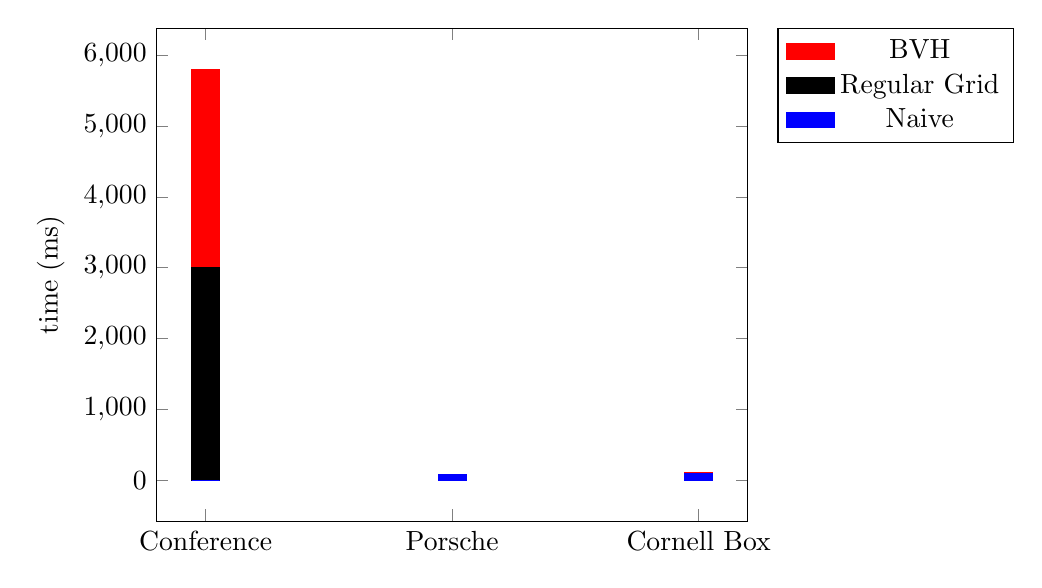
\begin{tikzpicture}
	\begin{axis}[
	legend style={at={(1.05,1.00)},anchor=north west},
	ylabel = time (ms),
	symbolic x coords={Conference, Porsche, Cornell Box},
	xtick=data,
	width=0.75\textwidth,
	]
	\addplot[ybar,fill=red,color=red,area legend] coordinates {
		(Conference,   0)
		(Conference,   5800)
		(Porsche,  	85)
		(Cornell Box,   105)
	};
	\addlegendentry{BVH}
	\addplot[ybar,fill=black,color=black,area legend] coordinates {
		(Conference,   0)
		(Conference,   3000)
		(Porsche,  	80)
		(Cornell Box,   99)
	};
	\addlegendentry{Regular Grid}
	\addplot[ybar,fill=blue,color=blue,area legend] coordinates {
		(Conference,   0)
		(Conference,   0)
		(Porsche,  	77)
		(Cornell Box,   91)
	};
	\addlegendentry{Naive}
	\end{axis}
	\label{graph:SamsungConstruct}
	\end{tikzpicture}
	\caption{Time to construct accelerators in the Samsung Galaxy smart phone}
\end{figure}

\begin{figure}[H]
	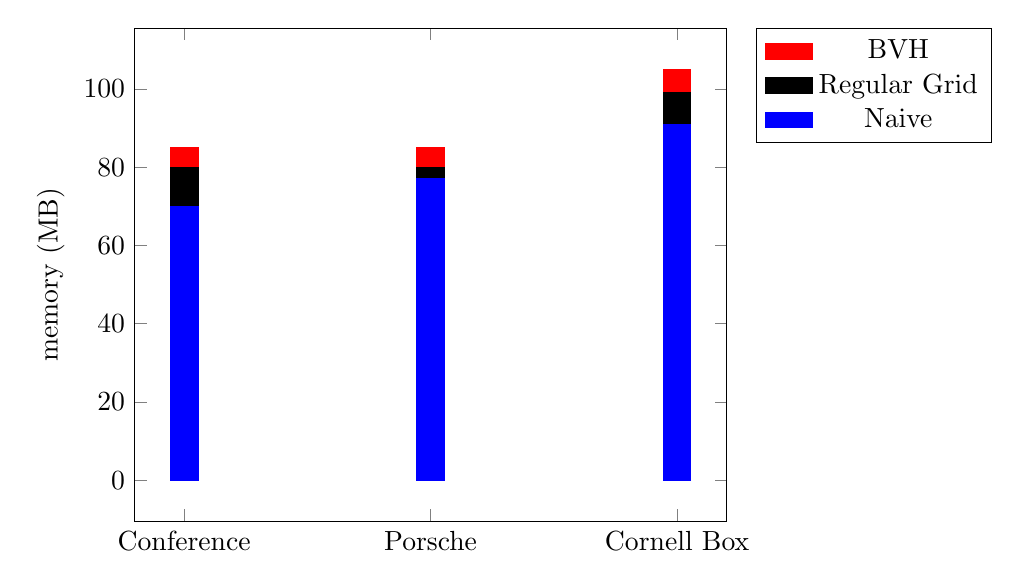
\begin{tikzpicture}
	\begin{axis}[
	legend style={at={(1.05,1.00)},anchor=north west},
	ylabel = memory (MB),
	symbolic x coords={Conference, Porsche, Cornell Box},
	xtick=data,
	width=0.75\textwidth,
	]
	\addplot[ybar,fill=red,color=red,area legend] coordinates {
		(Conference,   0)
		(Conference,   85)
		(Porsche,  	85)
		(Cornell Box,   105)
	};
	\addlegendentry{BVH}
	\addplot[ybar,fill=black,color=black,area legend] coordinates {
		(Conference,   0)
		(Conference,   80)
		(Porsche,  	80)
		(Cornell Box,   99)
	};
	\addlegendentry{Regular Grid}
	\addplot[ybar,fill=blue,color=blue,area legend] coordinates {
		(Conference,   0)
		(Conference,   70)
		(Porsche,  	77)
		(Cornell Box,   91)
	};
	\addlegendentry{Naive}
	\end{axis}
	\label{graph:SamsungMemory}
	\end{tikzpicture}
	\caption{Memory usage in the Samsung Galaxy smart phone}
\end{figure}

\subsubsection{Raspberry Pi 2 Model B}

\begin{figure}[H]
	\begin{tikzpicture}
	\begin{axis}[
	legend style={at={(1.05,1.00)},anchor=north west},
	axis lines = left,
	xlabel = \#threads,
	ylabel = time (ms),
	xtick={0,1,2,3,4},
	ytick={0,1,...,10},
	width=0.75\textwidth,
	]
	\addplot [
	color=blue,
	mark=*,
	dashed,
	] plot coordinates {
		(0,0.0)
		(1,1.0)
		(2,1.0)
		(3,1.0)
		(4,1.0)
	};
	\addlegendentry{Naive}
	\addplot [
	color=black,
	mark=*,
	dashed,
	] plot coordinates {
		(0,0.0)
		(1,1.0)
		(2,1.0)
		(3,1.0)
		(4,1.0)
	};
	\addlegendentry{Regular Grid}
	\addplot [
	color=red,
	mark=*,
	dashed,
	] plot coordinates {
		(0,0.0)
		(1,1.0)
		(2,1.0)
		(3,1.0)
		(4,1.0)
	};
	\addlegendentry{BVH}
	\label{graph:RaspberryTime}
	\end{axis}
	\end{tikzpicture}
\end{figure}

\begin{figure}[H]
	\begin{tikzpicture}
	\begin{axis}[
	legend style={at={(1.05,1.00)},anchor=north west},
	axis lines = left,
	xlabel = \#threads,
	ylabel = speedup,
	xtick={0,1,2,3,4},
	ytick={0,1,...,10},
	width=0.75\textwidth,
	]
	\addplot [
	color=blue,
	mark=*,
	dashed,
	] plot coordinates {
		(0,0.0)
		(1,1.0)
		(2,1.0)
		(3,1.0)
		(4,1.0)
	};
	\addlegendentry{Naive}
	\addplot [
	color=black,
	mark=*,
	dashed,
	] plot coordinates {
		(0,0.0)
		(1,1.0)
		(2,1.0)
		(3,1.0)
		(4,1.0)
	};
	\addlegendentry{Regular Grid}
	\addplot [
	color=red,
	mark=*,
	dashed,
	] plot coordinates {
		(0,0.0)
		(1,1.0)
		(2,1.0)
		(3,1.0)
		(4,1.0)
	};
	\addlegendentry{BVH}
	\label{graph:RaspberrySpeedup}
	\end{axis}
	\end{tikzpicture}
\end{figure}

\begin{figure}[H]
	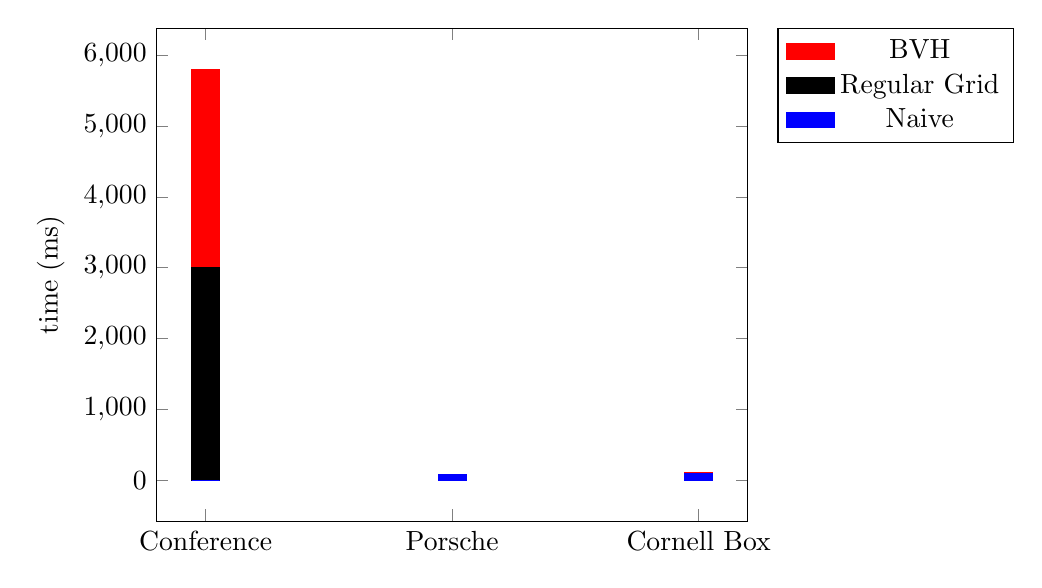
\begin{tikzpicture}
	\begin{axis}[
	legend style={at={(1.05,1.00)},anchor=north west},
	ylabel = time (ms),
	symbolic x coords={Conference, Porsche, Cornell Box},
	xtick=data,
	width=0.75\textwidth,
	]
	\addplot[ybar,fill=red,color=red,area legend] coordinates {
		(Conference,   0)
		(Conference,   5800)
		(Porsche,  	85)
		(Cornell Box,   105)
	};
	\addlegendentry{BVH}
	\addplot[ybar,fill=black,color=black,area legend] coordinates {
		(Conference,   0)
		(Conference,   3000)
		(Porsche,  	80)
		(Cornell Box,   99)
	};
	\addlegendentry{Regular Grid}
	\addplot[ybar,fill=blue,color=blue,area legend] coordinates {
		(Conference,   0)
		(Conference,   0)
		(Porsche,  	77)
		(Cornell Box,   91)
	};
	\addlegendentry{Naive}
	\end{axis}
	\label{graph:RaspberryConstruct}
	\end{tikzpicture}
	\caption{Time to construct accelerators in the Raspberry Pi 2 Model B}
\end{figure}

\begin{figure}[H]
	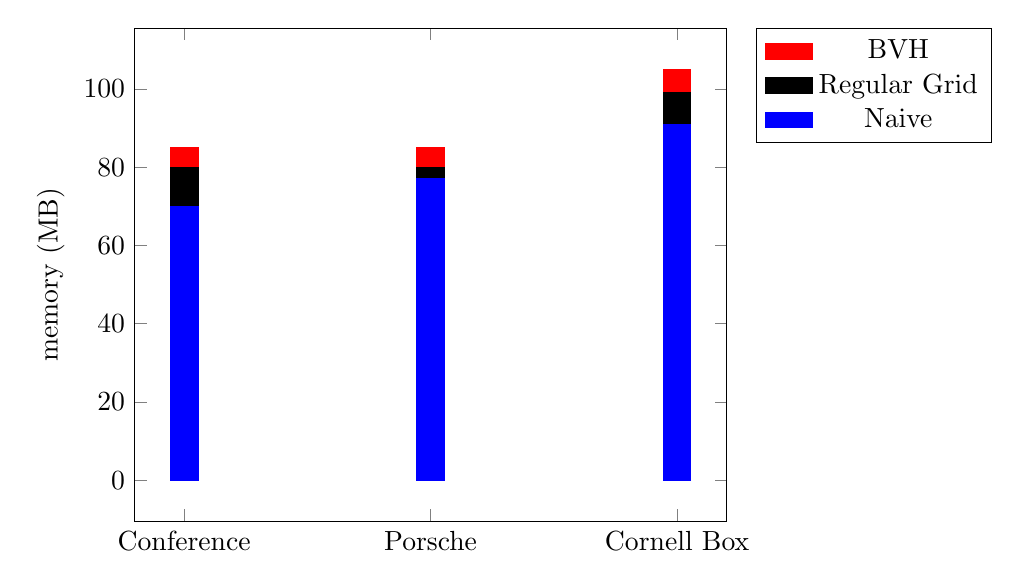
\begin{tikzpicture}
	\begin{axis}[
	legend style={at={(1.05,1.00)},anchor=north west},
	ylabel = memory (MB),
	symbolic x coords={Conference, Porsche, Cornell Box},
	xtick=data,
	width=0.75\textwidth,
	]
	\addplot[ybar,fill=red,color=red,area legend] coordinates {
		(Conference,   0)
		(Conference,   85)
		(Porsche,  	85)
		(Cornell Box,   105)
	};
	\addlegendentry{BVH}
	\addplot[ybar,fill=black,color=black,area legend] coordinates {
		(Conference,   0)
		(Conference,   80)
		(Porsche,  	80)
		(Cornell Box,   99)
	};
	\addlegendentry{Regular Grid}
	\addplot[ybar,fill=blue,color=blue,area legend] coordinates {
		(Conference,   0)
		(Conference,   70)
		(Porsche,  	77)
		(Cornell Box,   91)
	};
	\addlegendentry{Naive}
	\end{axis}
	\label{graph:RaspberryMemory}
	\end{tikzpicture}
	\caption{Memory usage in the Raspberry Pi 2 Model B}
\end{figure}


\subsubsection{MINIX NEO X8-H PLUS}

\begin{figure}[H]
	\begin{tikzpicture}
	\begin{axis}[
	legend style={at={(1.05,1.00)},anchor=north west},
	axis lines = left,
	xlabel = \#threads,
	ylabel = time (ms),
	xtick={0,1,2,3,4},
	ytick={0,1,...,10},
	width=0.75\textwidth,
	]
	\addplot [
	color=blue,
	mark=*,
	dashed,
	] plot coordinates {
		(0,0.0)
		(1,1.0)
		(2,1.0)
		(3,1.0)
		(4,1.0)
	};
	\addlegendentry{Naive}
	\addplot [
	color=black,
	mark=*,
	dashed,
	] plot coordinates {
		(0,0.0)
		(1,1.0)
		(2,1.0)
		(3,1.0)
		(4,1.0)
	};
	\addlegendentry{Regular Grid}
	\addplot [
	color=red,
	mark=*,
	dashed,
	] plot coordinates {
		(0,0.0)
		(1,1.0)
		(2,1.0)
		(3,1.0)
		(4,1.0)
	};
	\addlegendentry{BVH}
	\label{graph:MinixTime}
	\end{axis}
	\end{tikzpicture}
\end{figure}

\begin{figure}[H]
	\begin{tikzpicture}
	\begin{axis}[
	legend style={at={(1.05,1.00)},anchor=north west},
	axis lines = left,
	xlabel = \#threads,
	ylabel = speedup,
	xtick={0,1,2,3,4},
	ytick={0,1,...,10},
	width=0.75\textwidth,
	]
	\addplot [
	color=blue,
	mark=*,
	dashed,
	] plot coordinates {
		(0,0.0)
		(1,1.0)
		(2,1.0)
		(3,1.0)
		(4,1.0)
	};
	\addlegendentry{Naive}
	\addplot [
	color=black,
	mark=*,
	dashed,
	] plot coordinates {
		(0,0.0)
		(1,1.0)
		(2,1.0)
		(3,1.0)
		(4,1.0)
	};
	\addlegendentry{Regular Grid}
	\addplot [
	color=red,
	mark=*,
	dashed,
	] plot coordinates {
		(0,0.0)
		(1,1.0)
		(2,1.0)
		(3,1.0)
		(4,1.0)
	};
	\addlegendentry{BVH}
	\label{graph:MinixSpeedup}
	\end{axis}
	\end{tikzpicture}
\end{figure}

\begin{figure}[H]
	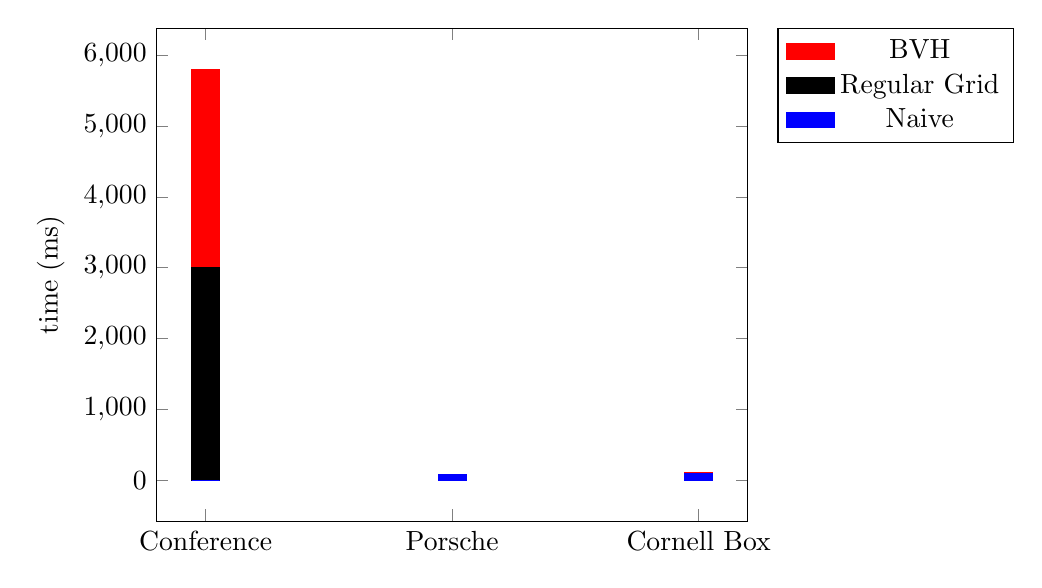
\begin{tikzpicture}
	\begin{axis}[
	legend style={at={(1.05,1.00)},anchor=north west},
	ylabel = time (ms),
	symbolic x coords={Conference, Porsche, Cornell Box},
	xtick=data,
	width=0.75\textwidth,
	]
	\addplot[ybar,fill=red,color=red,area legend] coordinates {
		(Conference,   0)
		(Conference,   5800)
		(Porsche,  	85)
		(Cornell Box,   105)
	};
	\addlegendentry{BVH}
	\addplot[ybar,fill=black,color=black,area legend] coordinates {
		(Conference,   0)
		(Conference,   3000)
		(Porsche,  	80)
		(Cornell Box,   99)
	};
	\addlegendentry{Regular Grid}
	\addplot[ybar,fill=blue,color=blue,area legend] coordinates {
		(Conference,   0)
		(Conference,   0)
		(Porsche,  	77)
		(Cornell Box,   91)
	};
	\addlegendentry{Naive}
	\end{axis}
	\label{graph:MinixConstruct}
	\end{tikzpicture}
	\caption{Time to construct accelerators in the MINIX NEO X8-H PLUS}
\end{figure}

\begin{figure}[H]
	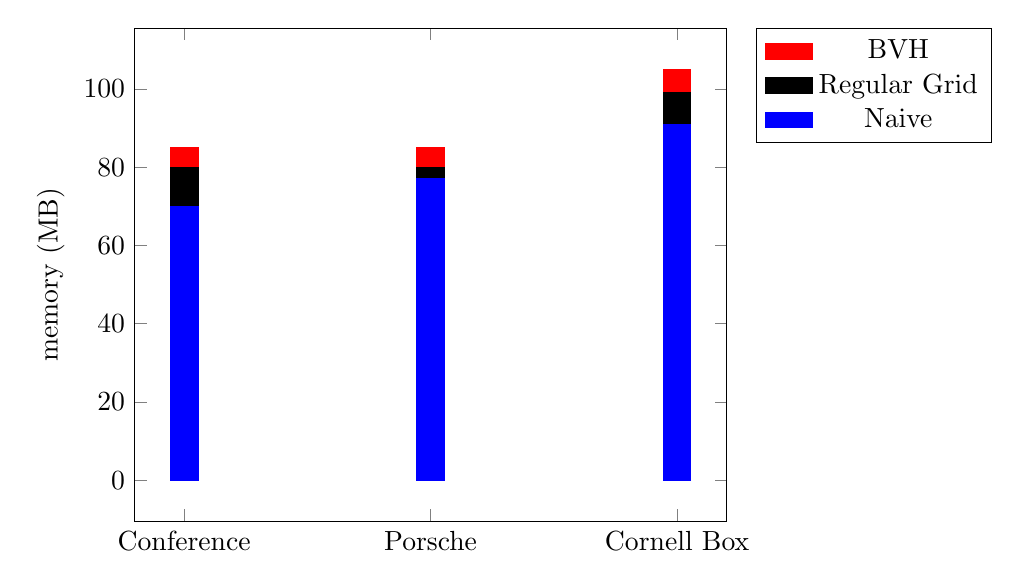
\begin{tikzpicture}
	\begin{axis}[
	legend style={at={(1.05,1.00)},anchor=north west},
	ylabel = memory (MB),
	symbolic x coords={Conference, Porsche, Cornell Box},
	xtick=data,
	width=0.75\textwidth,
	]
	\addplot[ybar,fill=red,color=red,area legend,width=4.30\textwidth] coordinates {
		(Conference,   0)
		(Conference,   85)
		(Porsche,  	85)
		(Cornell Box,   105)
	};
	\addlegendentry{BVH}
	\addplot[ybar,fill=black,color=black,area legend] coordinates {
		(Conference,   0)
		(Conference,   80)
		(Porsche,  	80)
		(Cornell Box,   99)
	};
	\addlegendentry{Regular Grid}
	\addplot[ybar,fill=blue,color=blue,area legend] coordinates {
		(Conference,   0)
		(Conference,   70)
		(Porsche,  	77)
		(Cornell Box,   91)
	};
	\addlegendentry{Naive}
	\end{axis}
	\label{graph:MinixMemory}
	\end{tikzpicture}
	\caption{Memory usage in the MINIX NEO X8-H PLUS}
\end{figure}

\section{Comparison with Android CPU Raytracer (\cite{Android_CPU_Raytracer})}

\par
Comparison ...

% Chapter - Conclusion/Future Work --------------
% CHAPTER - dizer que aprendi a fazer um ray tracer do zero
% CHAPTER - dizer que aprendi a fazer uma aplicaçao android
% CHAPTER - falar de possiveis componentes/estruturas de aceleraçao a implementar
% Tentar chegar às 50 páginas antes do capítulo 5
\chapter{Conclusion \& Future work}

\section{Conclusions}

\par
The constant evolution of technology allowed to leverage and massify the mobile devices.
With, more and increasingly powerful, mobile devices, it is possible to perform more and more complex and useful tasks in them.
This is a huge market where the programmers can develop their applications to, and where the development time can be a huge factor in their career success.

\par
But as noted in the section \ref{RelatedWork}, there is clearly a lack of well documented rendering libraries for mobile systems.
There is then the need to change this reality, since more and more the Internet of Things is more present each passing year, because there are increasingly powerful mobile systems.

\par
During the development of this ray tracer library, it was identified some challenges caused by the fact that it was developed for an Android mobile device, like, the smaller amount of RAM available for the software applications.
And, also, the simpler CPUs microarchitectures and smaller computational power available from these devices can make computational demanding applications, like ray tracers, difficult to perform the required calculations in a useful time for the user.
This fact is corroborated by the obtained results as demonstrated in section \ref{ResultsObtained}.

\section{Future Work}

\par
With respect to future work, it should be the development of the library for Android and the analysis of possibilities and challenges that may arise.
Upon completion of the development process, besides writing the dissertation and the article, it is expected to provide a demo application in order to illustrate the functionalities and performance that the library will offer.

\par
The library was implemented as planned, having been developed:


\begin{itemize}
	\item two acceleration structures
	\item three primitive shapes
	\item intersection
	\item material
	\item primitive
	\item ray
	\item renderer
	\item scene
	\item possibility to develop different types of cameras
	\item possibility to develop different types of lights
	\item possibility to develop different types of object loaders
	\item possibility to develop different types of samplers
	\item possibility to develop different types of shaders
\end{itemize}

\par
All these developed components allow the execution of the basic features of a ray tracer, such as the intersection of rays with the different shapes of primitives.
Besides that, it allows the user the possibility to develop several types of rendering components, like cameras, lights, object loaders, samplers and shaders.
With this, the user can create simple rendering applications that just use the rendering components offered together with the library, or even very complex applications, that use rendering components developed by the user.

\par
Besides the library, it was also developed several rendering components:

\begin{itemize}
	\item two cameras
	\item two lights
	\item one object loader
	\item six samplers
	\item five shaders
\end{itemize}

\par
This allows the user to develop rendering applications in an easy, safe and fast way, as was intended in this dissertation.
Unfortunately, this does not allow rapid development of all kinds of rendering applications.
One of the things that can be improved in this library is allowing to put more than one camera in the scene, so that you can cast rays to the scene from more than one different point.
And thus open the possibility of allowing the user to develop more different shaders, such as Bidirectional Path Tracing, or even allowing to render the 3D scene into a 3D image.

\par
Other thing that could be implemented is a texture loader for the ray tracer.
This allows the possibility to render more beautiful scenes.

\par
And last but not least, there is always the possibility to improve the ray tracer performance by redeveloping the application using a 
Data-oriented design instead of the traditional Object-oriented design used.
This approach approach was motivated by cache coherency, used in video game development, usually in the programming languages C or C++.

%- Bibliography (needs bibtex) -%
\bibliography{dissertation}
\nocite {*}

\begin{appendices}
\chapter{User documentation}

\section{API}

\par

\begin{lstlisting}[caption={Renderer API}, captionpos=b, label=API_Renderer]
public:
explicit Renderer(::std::unique_ptr<Shader> shader,
	::std::unique_ptr<Camera> camera,
	::std::unique_ptr<Sampler> samplerPixel,
	::std::uint32_t width, ::std::uint32_t height,
	::std::uint32_t samplesPixel) noexcept;

Renderer(const Renderer &renderer) noexcept = delete;

Renderer(Renderer &&renderer) noexcept = delete;

~Renderer() noexcept = default;

Renderer &operator=(const Renderer &renderer) noexcept = delete;

Renderer &operator=(Renderer &&renderer) noexcept = delete;

void renderFrame(::std::uint32_t *bitmap, ::std::int32_t numThreads, ::std::uint32_t stride) noexcept;

void stopRender() noexcept;

::std::uint32_t getSample() const noexcept;
\end{lstlisting}

\begin{lstlisting}[caption={Scene API}, captionpos=b, label=API_Scene]
public:
explicit Scene() = default;

Scene(const Scene &scene) noexcept = delete;

Scene(Scene &&scene) noexcept = default;

~Scene() noexcept;

Scene &operator=(const Scene &scene) noexcept = delete;

Scene &operator=(Scene &&scene) noexcept = default;

Intersection trace(Intersection intersection, const Ray &ray) noexcept;

Intersection shadowTrace(Intersection intersection, const Ray &ray) noexcept;

Intersection traceLights(Intersection intersection, const Ray &ray) const noexcept;

void resetSampling() noexcept;
\end{lstlisting}

\begin{lstlisting}[caption={Ray API}, captionpos=b, label=API_Ray]
public:
explicit Ray(const ::glm::vec3 &dir, const ::glm::vec3 &origin,
::std::int32_t depth, const void *primitive = nullptr) noexcept;

Ray(const Ray &ray) noexcept = default;

Ray(Ray &&ray) noexcept = default;

~Ray() noexcept = default;

Ray &operator=(const Ray &ray) noexcept = delete;

Ray &operator=(Ray &&ray) noexcept = delete;
\end{lstlisting}

\begin{lstlisting}[caption={Primitive API}, captionpos=b, label=API_Primitive]
public:
Primitive(const T &shape, const Material &material) noexcept;

Primitive() noexcept = delete;

Primitive(const Primitive &primitive) noexcept = default;

Primitive(Primitive &&primitive) noexcept = default;

~Primitive() noexcept = default;

Primitive &operator=(const Primitive &primitive) noexcept = default;

Primitive &operator=(Primitive &&primitive) noexcept = default;

AABB getAABB() const noexcept;

Intersection intersect(Intersection intersection, const Ray &ray) noexcept;
\end{lstlisting}

\begin{lstlisting}[caption={Intersection API}, captionpos=b, label=API_Intersection]
public:
explicit Intersection() noexcept = default;

explicit Intersection(float dist, const void *primitive = nullptr) noexcept;

explicit Intersection(
	const ::glm::vec3 &orig,
	const ::glm::vec3 &dir,
	float dist,
	const ::glm::vec3 &normal,
	const void *primitive = nullptr) noexcept;

explicit Intersection(
	const ::glm::vec3 &intPoint,
	float dist,
	const ::glm::vec3 &sphereCenter) noexcept;

Intersection(const Intersection &intersection) noexcept = default;

Intersection(Intersection &&intersection) noexcept = default;

~Intersection() noexcept = default;

Intersection &operator=(const Intersection &intersection) noexcept = delete;

Intersection &operator=(Intersection &&intersection) noexcept = default;
\end{lstlisting}

\begin{lstlisting}[caption={Material API}, captionpos=b, label=API_Material]
public:
explicit Material(
	const ::glm::vec3 &Kd = ::glm::vec3 {},
	const ::glm::vec3 &Ks = ::glm::vec3 {},
	const ::glm::vec3 &Kt = ::glm::vec3 {},
	float refractiveIndice = 1.0f, const ::glm::vec3 &Le = ::glm::vec3 {}) noexcept;

Material(const Material &material) noexcept = default;

Material(Material &&material) noexcept = default;

~Material() noexcept = default;

Material &operator=(const Material &material) noexcept = default;

Material &operator=(Material &&material) noexcept = default;
\end{lstlisting}

\begin{lstlisting}[caption={Triangle API}, captionpos=b, label=API_Triangle]
public:
explicit Triangle(
	const ::glm::vec3 &pointA, const ::glm::vec3 &pointB, const ::glm::vec3 &pointC,
	const ::glm::vec3 &normal = ::glm::vec3 {}) noexcept;

Triangle(const Triangle &triangle) noexcept = default;

Triangle(Triangle &&triangle) noexcept = default;

~Triangle() noexcept = default;

Triangle &operator=(const Triangle &triangle) noexcept = default;

Triangle &operator=(Triangle &&triangle) noexcept = default;

Intersection intersect(const Intersection &intersection, const Ray &ray) const noexcept;

void moveTo(float x, float y) noexcept;

float getZ() const noexcept;

AABB getAABB() const noexcept;

bool intersect(const AABB &box) const noexcept;
\end{lstlisting}

\begin{lstlisting}[caption={Plane API}, captionpos=b, label=API_Plane]
public:
explicit Plane(const ::glm::vec3 &point, const ::glm::vec3 &normal) noexcept;

Plane(const Plane &plane) noexcept = default;

Plane(Plane &&plane) noexcept = default;

~Plane() noexcept = default;

Plane &operator=(const Plane &plane) noexcept = default;

Plane &operator=(Plane &&plane) noexcept = default;

Intersection intersect(const Intersection &intersection, const Ray &ray) const noexcept;

void moveTo(float x, float y) noexcept;

float getZ() const noexcept;

AABB getAABB() const noexcept;

float distance(const ::glm::vec3 &point) const noexcept;

bool intersect(const AABB &box) const noexcept;
\end{lstlisting}

\begin{lstlisting}[caption={Sphere API}, captionpos=b, label=API_Sphere]
public:
explicit Sphere(const ::glm::vec3 &center, float radius) noexcept;

Sphere(const Sphere &sphere) noexcept = default;

Sphere(Sphere &&sphere) noexcept = default;

~Sphere() noexcept = default;

Sphere &operator=(const Sphere &sphere) noexcept = default;

Sphere &operator=(Sphere &&sphere) noexcept = default;

Intersection intersect(const Intersection &intersection, const Ray &ray) const noexcept;

void moveTo(float x, float y) noexcept;

float getZ() const noexcept;

AABB getAABB() const noexcept;

bool intersect(const AABB &box) const noexcept;
\end{lstlisting}


\begin{lstlisting}[caption={Utils API}, captionpos=b, label=API_Utils]
#define LOG(...) {::MobileRT::log(::MobileRT::getFileName(__FILE__), ":", __LINE__, ": ",
__VA_ARGS__);}

template<typename ...Args>
void log(Args &&... args) noexcept;

inline ::std::string getFileName(const char *filepath) noexcept;

template<typename T>
::std::vector<T *> convertVector(::std::vector<T> &source) noexcept;

::std::int32_t roundDownToMultipleOf(::std::int32_t value, ::std::int32_t multiple) noexcept;

float haltonSequence(::std::uint32_t index, ::std::uint32_t base) noexcept;

::std::uint32_t incrementalAvg(
	const ::glm::vec3 &sample, ::std::uint32_t avg, ::std::uint32_t numSample) noexcept;
\end{lstlisting}

\begin{lstlisting}[caption={AABB API}, captionpos=b, label=API_AABB]
public:
explicit AABB() noexcept = default;

explicit AABB(const ::glm::vec3 &pointMin, const ::glm::vec3 &pointMax) noexcept;

AABB(const AABB &AABB) noexcept = default;

AABB(AABB &&AABB) noexcept = default;

~AABB() noexcept = default;

AABB &operator=(const AABB &AABB) noexcept = default;

AABB &operator=(AABB &&AABB) noexcept = default;

float getSurfaceArea() const noexcept;

::std::int32_t getLongestAxis() const noexcept;
\end{lstlisting}

\begin{lstlisting}[caption={BVH API}, captionpos=b, label=API_BVH]
public:
explicit BVH() noexcept = default;

explicit BVH<T>(
	::std::vector<Primitive<T>> &&primitives) noexcept;

BVH(const BVH &bVH) noexcept = delete;

BVH(BVH &&bVH) noexcept = default;

~BVH() noexcept = default;

BVH &operator=(const BVH &bVH) noexcept = delete;

BVH &operator=(BVH &&bVH) noexcept = default;

Intersection trace(Intersection intersection, const Ray &ray) noexcept;

Intersection shadowTrace(Intersection intersection, const Ray &ray) noexcept;
\end{lstlisting}

\begin{lstlisting}[caption={RegularGrid API}, captionpos=b, label=API_RegularGrid]
public:
explicit RegularGrid() noexcept = default;

explicit RegularGrid(AABB sceneBounds, Scene *scene, ::std::int32_t gridSize) noexcept;

RegularGrid(const RegularGrid &regularGrid) noexcept = delete;

RegularGrid(RegularGrid &&regularGrid) noexcept = default;

~RegularGrid() noexcept = default;

RegularGrid &operator=(const RegularGrid &regularGrid) noexcept = delete;

RegularGrid &operator=(RegularGrid &&regularGrid) noexcept = default;

Intersection trace(Intersection intersection, const Ray &ray) noexcept;

Intersection shadowTrace(Intersection intersection, const Ray &ray) noexcept;
\end{lstlisting}


\begin{lstlisting}[caption={Shader API}, captionpos=b, label=API_Shader]
protected:
virtual bool shade(::glm::vec3 *rgb, const Intersection &intersection,
const Ray &ray) noexcept = 0;

::glm::vec3 getCosineSampleHemisphere(const ::glm::vec3 &normal) const noexcept;

public:
void initializeAccelerators(Camera *camera) noexcept;

public:
explicit Shader(Scene scene, ::std::uint32_t samplesLight, Accelerator accelerator) noexcept;

Shader(const Shader &shader) noexcept = delete;

Shader(Shader &&shader) noexcept = default;

virtual ~Shader() noexcept;

Shader &operator=(const Shader &shader) noexcept = delete;

Shader &operator=(Shader &&shader) noexcept = delete;

bool rayTrace(::glm::vec3 *rgb, const Ray &ray) noexcept;

bool shadowTrace(Intersection intersection, const Ray &ray) noexcept;

Intersection traceTouch(Intersection intersection, const Ray &ray) noexcept;

virtual void resetSampling() noexcept;

::std::uint32_t getLightIndex ();
\end{lstlisting}

\begin{lstlisting}[caption={Sampler API}, captionpos=b, label=API_Sampler]
public:
explicit Sampler() noexcept = default;

explicit Sampler(::std::uint32_t width, ::std::uint32_t height,
::std::uint32_t samples) noexcept;

Sampler(const Sampler &sampler) noexcept = delete;

Sampler(Sampler &&sampler) noexcept = delete;

virtual ~Sampler() noexcept;

Sampler &operator=(const Sampler &sampler) noexcept = delete;

Sampler &operator=(Sampler &&sampler) noexcept = delete;

void resetSampling() noexcept;

void stopSampling() noexcept;

virtual float getSample(::std::uint32_t sample) noexcept = 0;

float getSample() noexcept;
\end{lstlisting}

\begin{lstlisting}[caption={Camera API}, captionpos=b, label=API_Camera]
protected:
float degToRad(const float deg) const noexcept;
float radToDeg(const float rad) const noexcept;

public:
explicit Camera(const ::glm::vec3 &position,
	const ::glm::vec3 &lookAt, const ::glm::vec3 &up) noexcept;

Camera(const Camera &camera) noexcept;

Camera(Camera &&camera) noexcept = delete;

virtual ~Camera() noexcept;

Camera &operator=(const Camera &camera) noexcept = delete;

Camera &operator=(Camera &&camera) noexcept = delete;

virtual Ray generateRay(float u, float v,
	float deviationU,
	float deviationV) const noexcept = 0;

float getBlock(::std::uint32_t sample) noexcept;

virtual AABB getAABB() const noexcept;

void resetSampling() noexcept;
\end{lstlisting}

\begin{lstlisting}[caption={Light API}, captionpos=b, label=API_Light]
public:
explicit Light(const Material &radiance) noexcept;

Light(const Light &light) noexcept = delete;

Light(Light &&light) noexcept = delete;

virtual ~Light() noexcept;

Light &operator=(const Light &light) noexcept = delete;

Light &operator=(Light &&light) noexcept = delete;

virtual ::glm::vec3 getPosition() noexcept = 0;

virtual void resetSampling() noexcept = 0;

virtual Intersection intersect(Intersection intersection, const Ray &ray) const noexcept = 0;
\end{lstlisting}

\begin{lstlisting}[caption={ObjectLoader API}, captionpos=b, label=API_ObjectLoader]
public:
explicit ObjectLoader() noexcept = default;

ObjectLoader(const ObjectLoader &objectLoader) noexcept = delete;

ObjectLoader(ObjectLoader &&objectLoader) noexcept = delete;

virtual ~ObjectLoader() noexcept;

ObjectLoader &operator=(const ObjectLoader &objectLoader) noexcept = delete;

ObjectLoader &operator=(ObjectLoader &&objectLoader) noexcept = delete;

virtual void process() noexcept = 0;

bool isProcessed() const noexcept;

virtual bool fillScene(Scene *scene,
::std::function<::std::unique_ptr<Sampler>()> lambda,
JNIEnv *env) noexcept = 0;
\end{lstlisting}

\section{Loading a scene}

\par


\begin{lstlisting}[caption={How to load a 3D scene}, captionpos=b, label=LoadingScene]
jboolean isCopy {JNI_FALSE};
const char *const objFileName {(env)->GetStringUTFChars(globalObjFile, &isCopy)};
const char *const matFileName {(env)->GetStringUTFChars(globalMatFile, &isCopy)};

const jboolean result{
	env->CallStaticBooleanMethod(mainActivityClass, mainActivityMethodId, 0)};
if (result) {
	return -1;
}

::Components::OBJLoader objLoader{objFileName, matFileName};
{
	const jboolean result{
	env->CallStaticBooleanMethod(mainActivityClass, mainActivityMethodId, 0)};
	if (result) {
		return -1;
	}
}
objLoader.process();
{
	const jboolean result{
	env->CallStaticBooleanMethod(mainActivityClass, mainActivityMethodId, 0)};
	if (result) {
		return -1;
	}
}

if (!objLoader.isProcessed()) {
	return -1;
}
const bool sceneBuilt{objLoader.fillScene(&scene_,
[]() { return ::std::make_unique<Components::StaticHaltonSeq>(); }, env)};
if (!sceneBuilt) {
	return -1;
}
{
	const jboolean result{
	env->CallStaticBooleanMethod(mainActivityClass, mainActivityMethodId, 0)};
	if (result) {
		return -1;
	}
}

const float ratio {
::std::max(static_cast<float>(width) / height, static_cast<float>(height) / width)};
const float hfovFactor{width > height ? ratio : 1.0f};
const float vfovFactor{width < height ? ratio : 1.0f};
const float fovX{45.0f * hfovFactor};
const float fovY{45.0f * vfovFactor};
maxDist = ::glm::vec3 {1, 1, 1};
const ::MobileRT::Material &lightMat{::glm::vec3 {0.0f, 0.0f, 0.0f},
	::glm::vec3 {0.0f, 0.0f, 0.0f},
	::glm::vec3 {0.0f, 0.0f, 0.0f},
	1.0f,
	::glm::vec3 {0.9f, 0.9f, 0.9f}};

//cornellbox
if (::std::strstr(objFileName, "CornellBox") != nullptr) {
	camera = ::std::make_unique<Components::Perspective>(
		::glm::vec3 {0.0f, 0.7f, 3.0f},
		::glm::vec3 {0.0f, 0.7f, -1.0f},
		::glm::vec3 {0.0f, 1.0f, 0.0f},
		fovX, fovY);
	
	::std::unique_ptr<MobileRT::Sampler> samplerPoint1{
	::std::make_unique<Components::StaticHaltonSeq>()};
	scene_.lights_.emplace_back(::std::make_unique<::Components::AreaLight>(
		lightMat,
		::std::move(samplerPoint1),
		::glm::vec3 {0.5f, 1.58f, 0.5f},
		::glm::vec3 {-0.5f, 1.58f, 0.5f},
		::glm::vec3 {-0.5f, 1.58f, -0.5f}));
	::std::unique_ptr<MobileRT::Sampler> samplerPoint2{
	::std::make_unique<Components::StaticHaltonSeq>()};
	scene_.lights_.emplace_back(::std::make_unique<::Components::AreaLight>(
		lightMat,
		::std::move(samplerPoint2),
		::glm::vec3 {0.5f, 1.58f, 0.5f},
		::glm::vec3 {-0.5f, 1.58f, -0.5f},
		::glm::vec3 {0.5f, 1.58f, -0.5f}));
}
\end{lstlisting}
\end{appendices}

\end{document}